%- - - - - - - - - - - - - - - - - - - - - - - - - - - - - - - - - SLIDE -
\begin{frame}
\frametitle{Competições de Programação}
\begin{block}{O que são?}
\begin{itemize}
	\item São competições onde um programador, ou grupo de programadores, deve apresentar soluções computacionais corretas para um dado conjunto de problemas.
	\begin{itemize}
		\item A correção é automatizada e realizada por meio de testes:
		\begin{itemize}
			\item um conjunto de dados de entrada.
			\item um meio de validar a resposta gerada.
		\end{itemize}
		\item O programa solução deve:
		\begin{itemize}
			\item gerar um conjunto de dados de saída correspondente ao conjunto de dados recebido na entrada.
			\item respeitar limites de tempo de execução e de quantidade de memória usada.
			\item o resultado do programa deve ser validado corretamente nos testes realizados.
		\end{itemize}
	\end{itemize}
\end{itemize}
\end{block}
\end{frame}
%- - - - - - - - - - - - - - - - - - - - - - - - - - - - - - - - - SLIDE -
\begin{frame}
\frametitle{Competições de Programação}
\begin{block}{Por que é Bom?}
\begin{itemize}
	\item Essas competições estimulam a capacidade de resolver problemas computacionais rápida e eficientemente, uma das principais habilidades exigidas de um profissional de Computação.
	\item Você ganha motivação para estudar algoritmos e estruturas de dados.
    \item Estimulam o raciocínio lógico, o que acaba resultando em um melhor desempenho acadêmico.
	\item Você busca conhecer todos os recursos das linguagens de programação.
	\item Possibilidade de viagem para vários destinos do Brasil e do mundo.
    \item Boas colocações nessas competições enriquecem seu curriculo como programador e resolvedor de problemas, o que é muito valorizado por grandes empresas da área.
	\item É sempre bom competir!
\end{itemize}
\end{block}
\end{frame}

%- - - - - - - - - - - - - - - - - - - - - - - - - - - - - - - - -
%- - - - - - - - - - - - - - - - - - - - - - - - - - - - - - - - - SLIDES - SNCT
\begin{frame}
\frametitle{Competições de Programação}
\begin{block}{Por que é Bom?}
\begin{center}
	
\includegraphics[height=.7\textheight]{sntc/IMG_1649.JPG}
\end{center}
\end{block}
\end{frame}
\begin{frame}
\frametitle{Competições de Programação}
\begin{block}{Por que é Bom?}
\begin{center}
	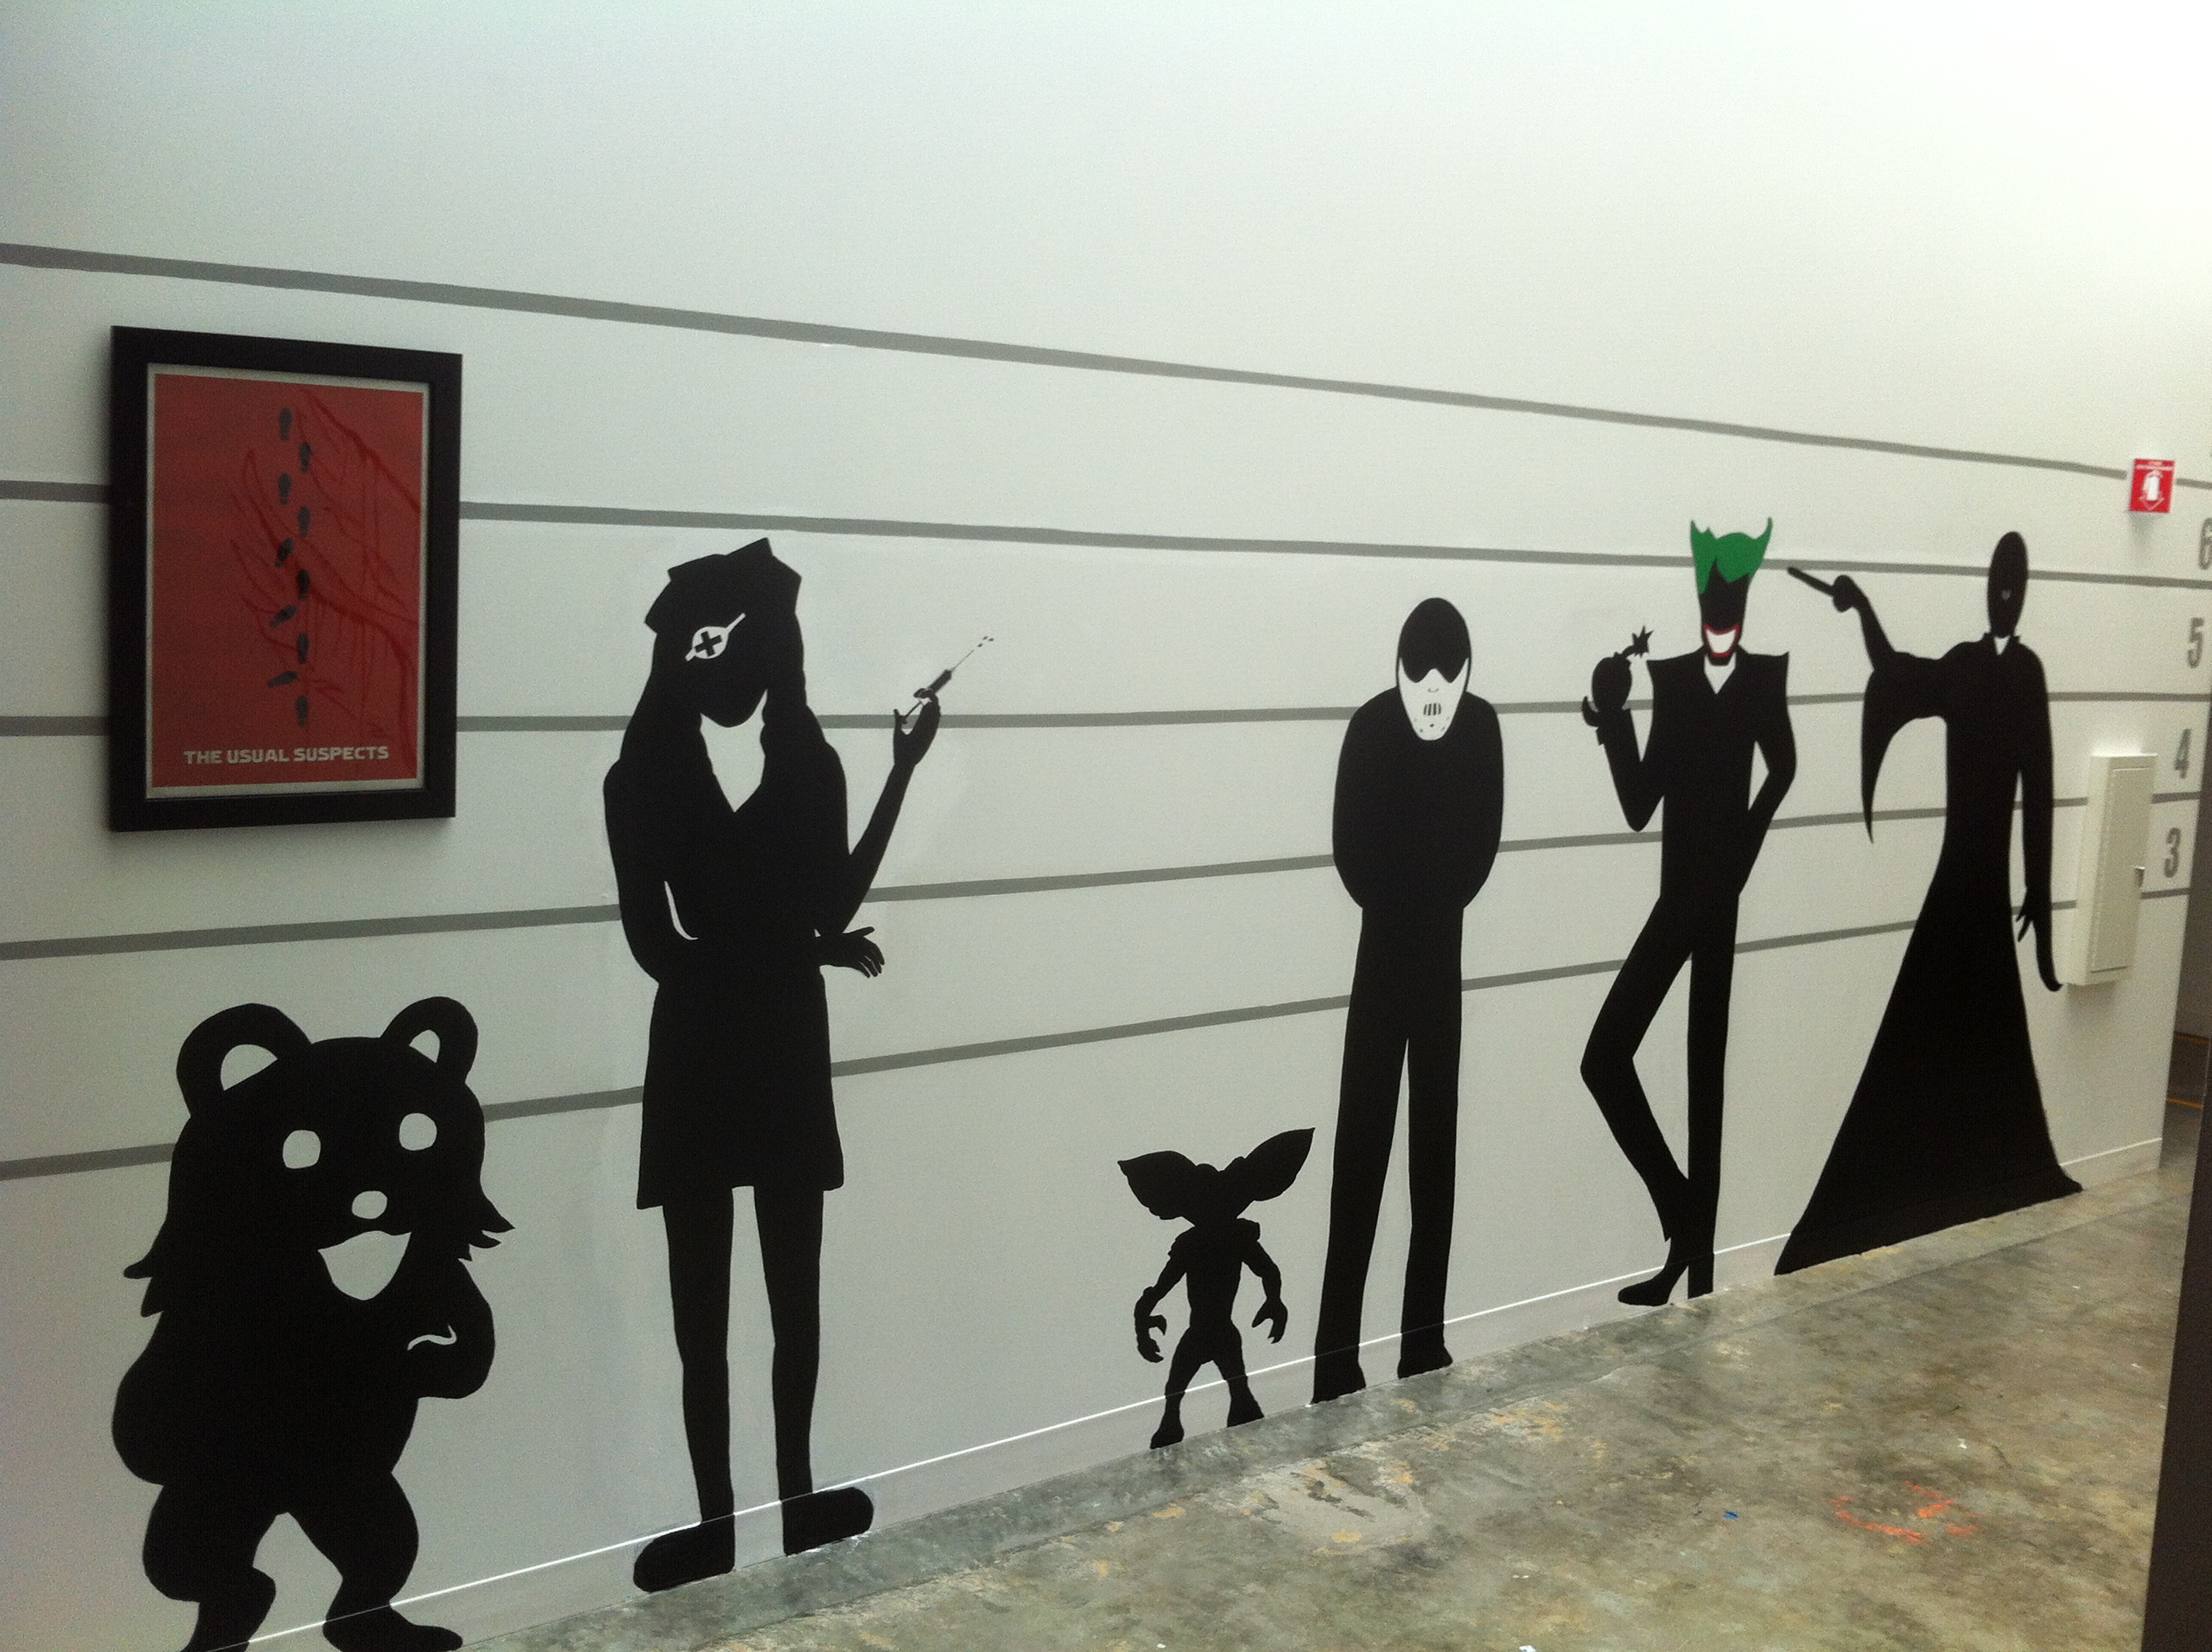
\includegraphics[width=.7\textwidth]{sntc/IMG_2040.JPG}
\end{center}
\end{block}
\end{frame}
\begin{frame}
\frametitle{Competições de Programação}
\begin{block}{Por que é Bom?}
\begin{center}
	
\includegraphics[width=.7\textwidth]{sntc/IMG_2045.JPG}
\end{center}
\end{block}
\end{frame}
\begin{frame}
\frametitle{Competições de Programação}
\begin{block}{\tiny{Por que é Bom?}}
\begin{center}
	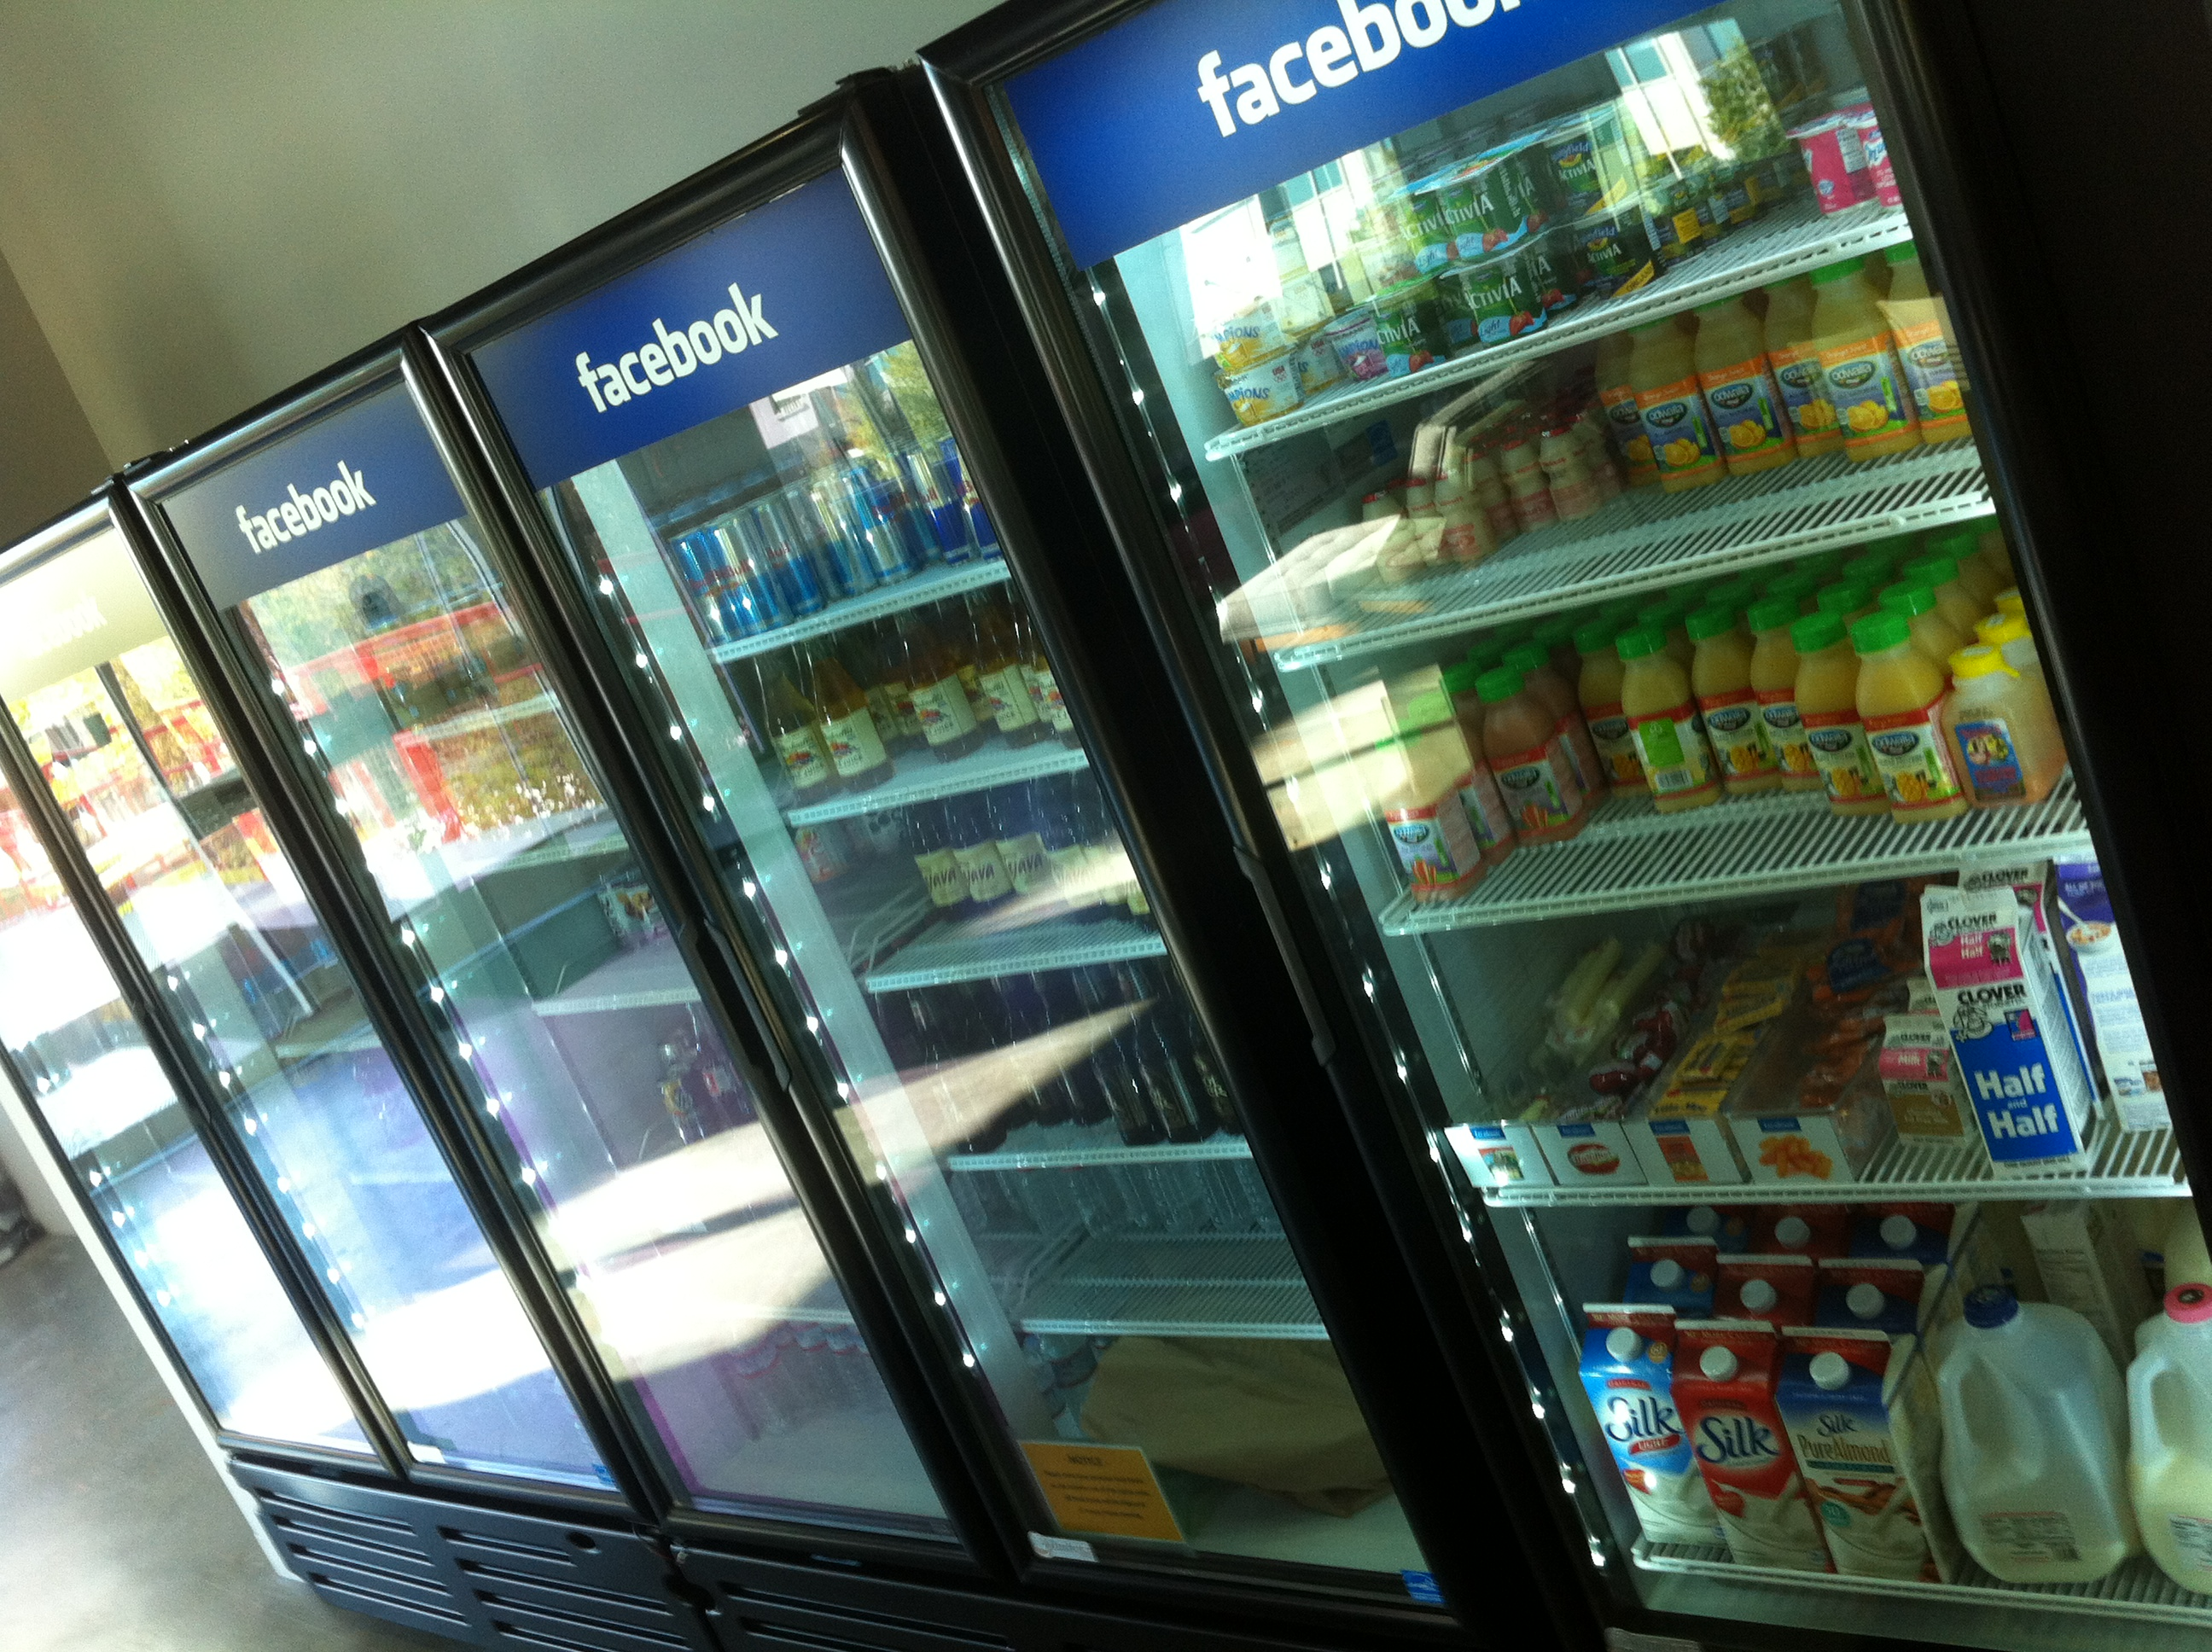
\includegraphics[width=.7\textwidth]{sntc/IMG_2049.JPG}
\end{center}
\end{block}
\end{frame}
\begin{frame}
\frametitle{Competições de Programação}
\begin{block}{Por que é Bom?}
\begin{center}
	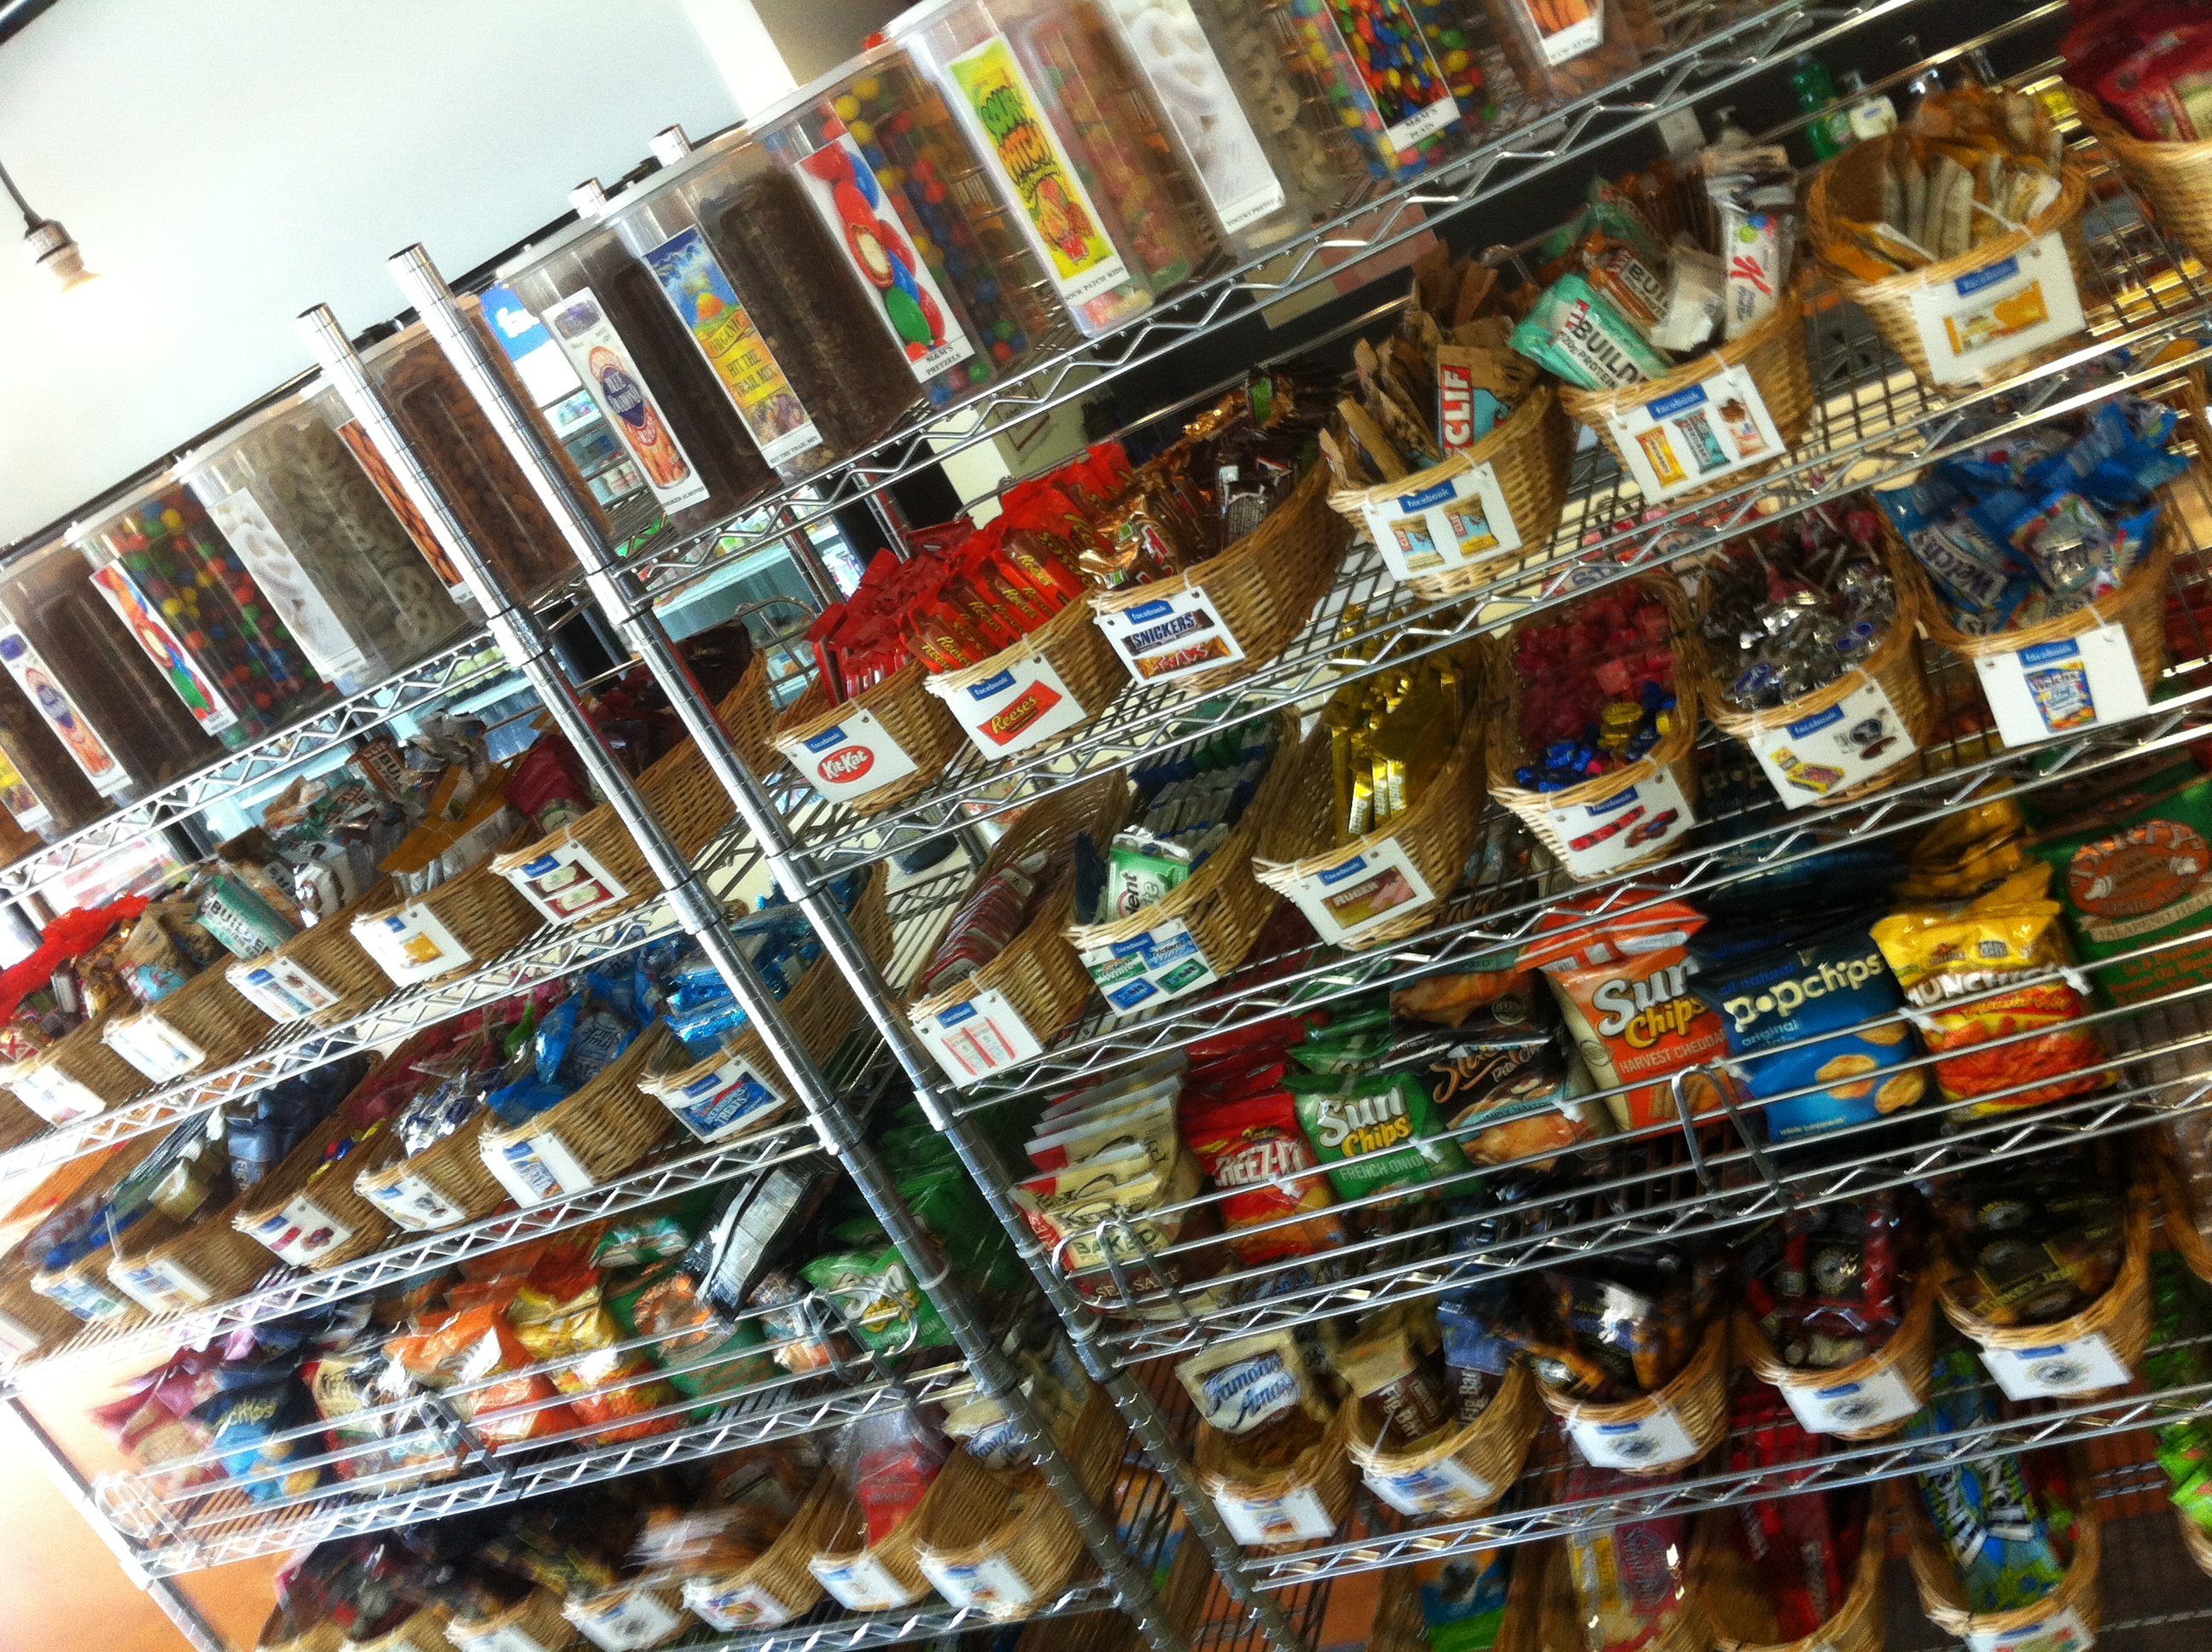
\includegraphics[width=.7\textwidth]{sntc/IMG_2050.JPG}
\end{center}
\end{block}
\end{frame}
\begin{frame}
\frametitle{Competições de Programação}
\begin{block}{Por que é Bom?}
\begin{center}
	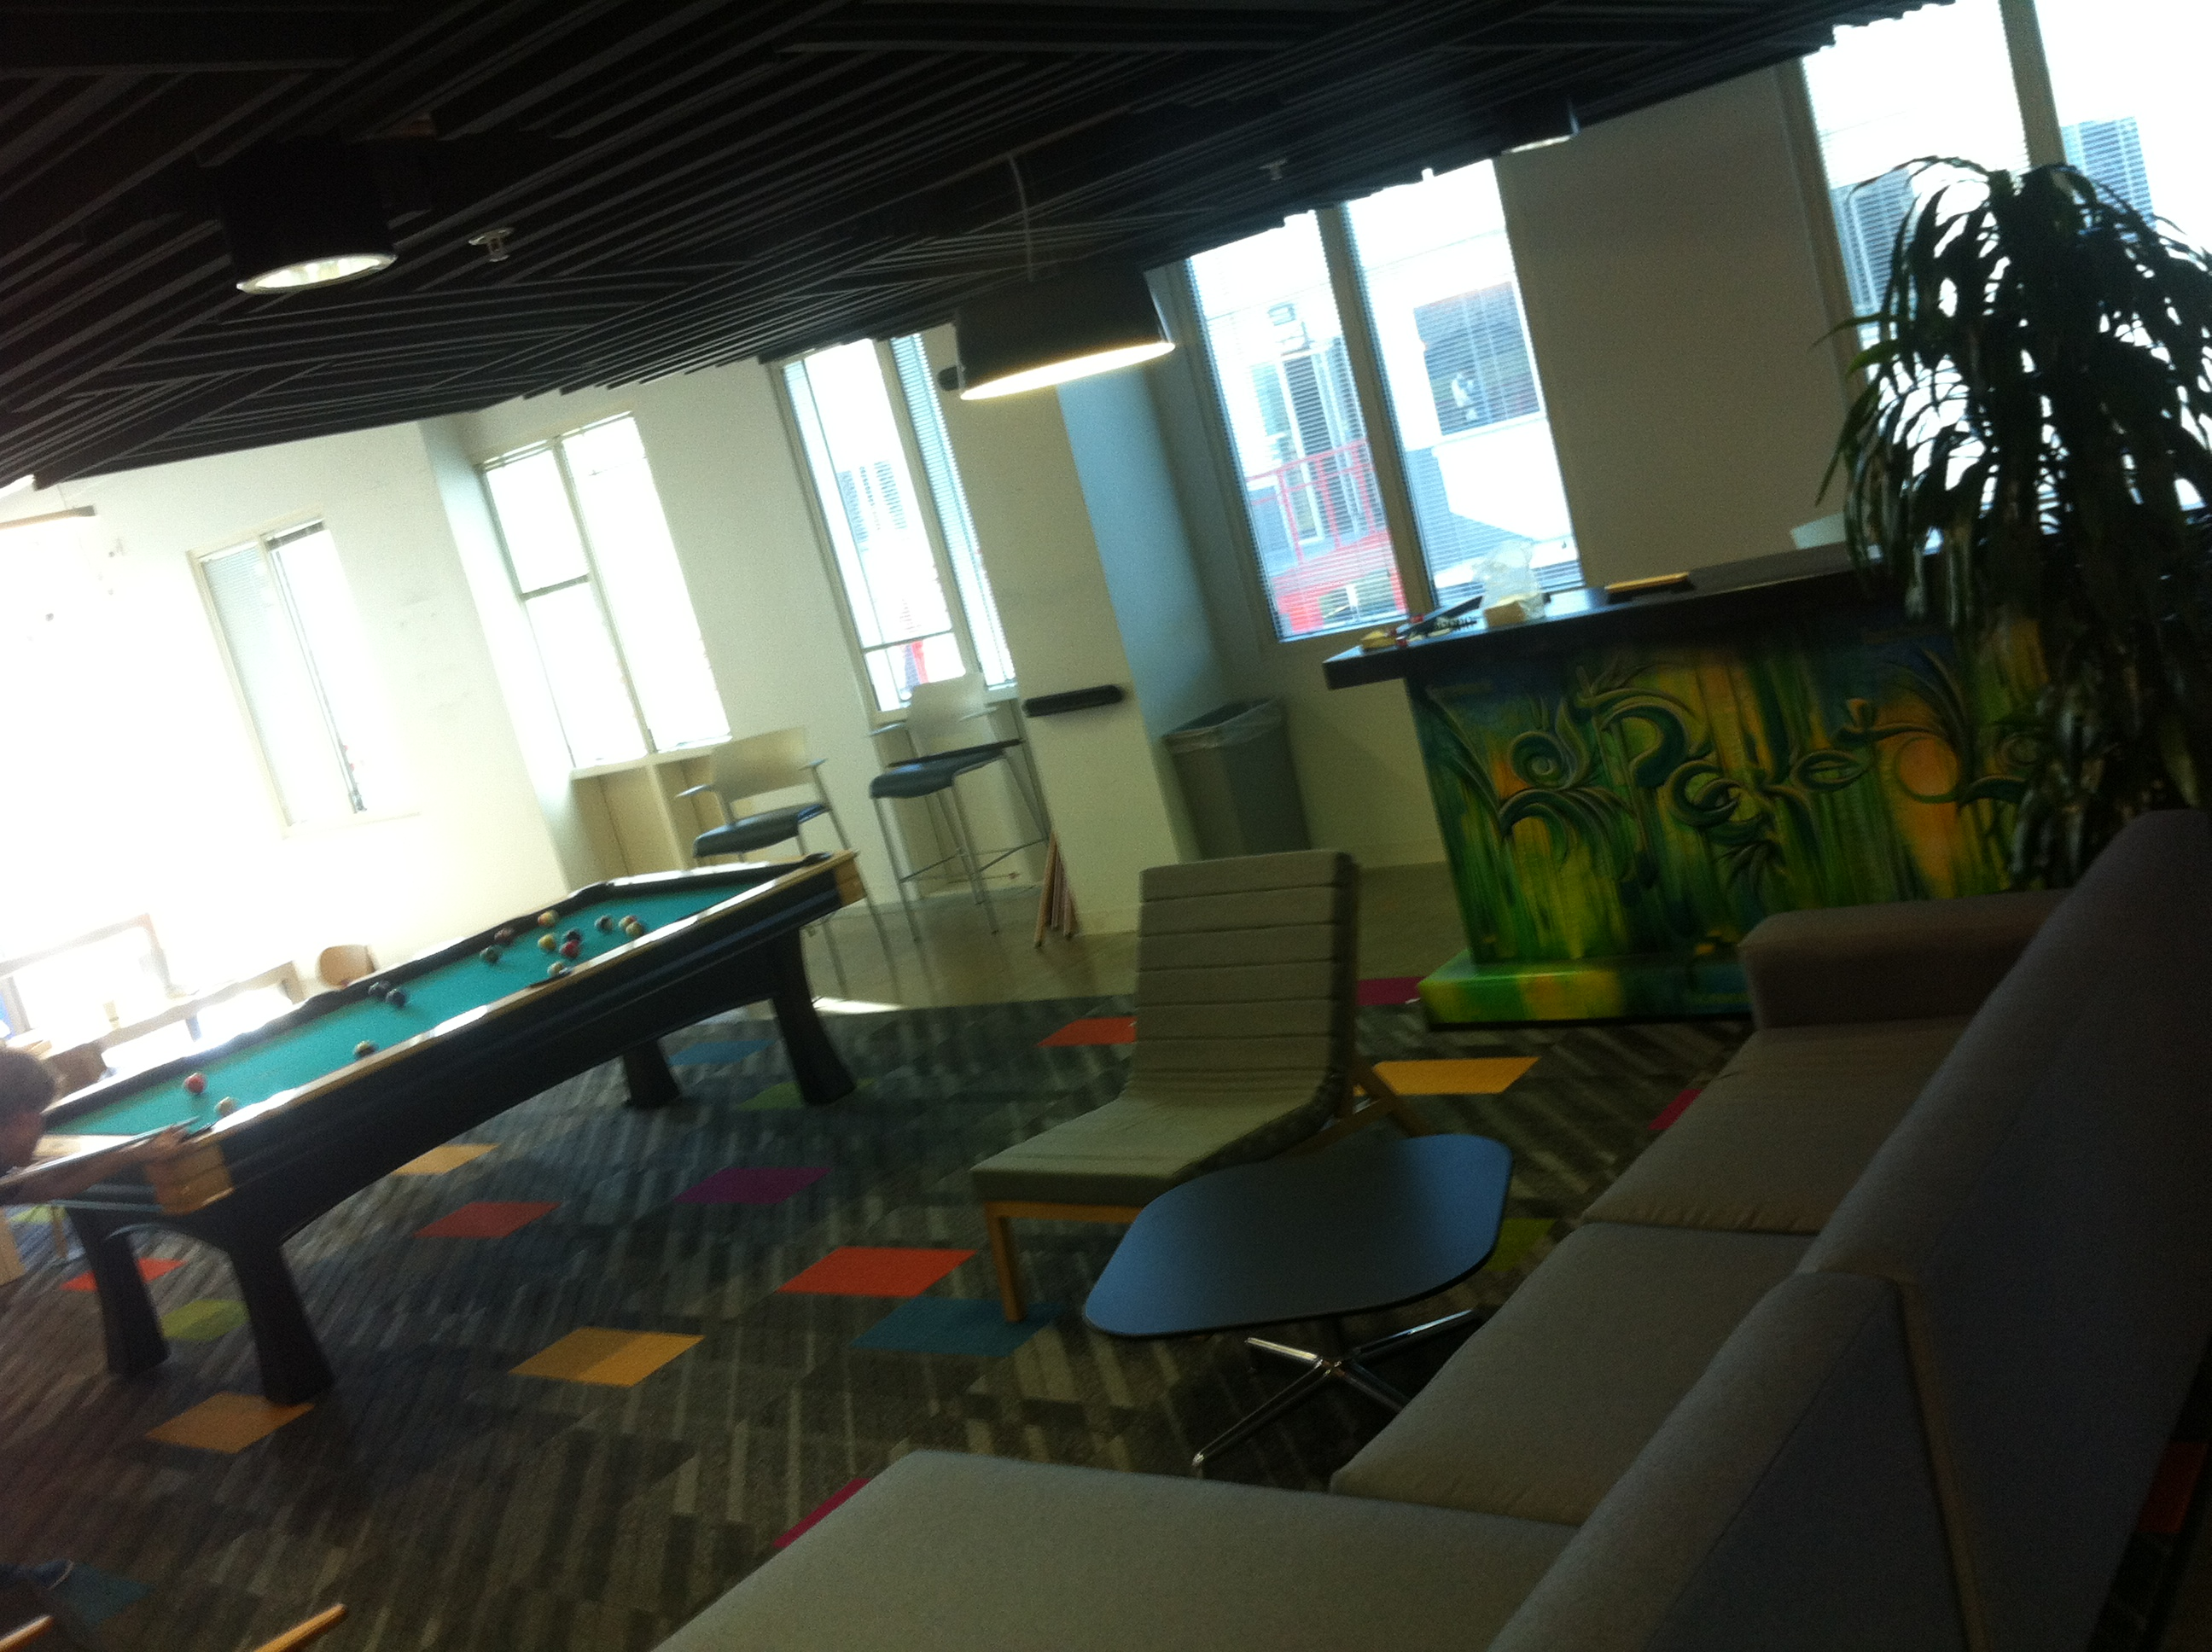
\includegraphics[width=.7\textwidth]{sntc/IMG_2051.JPG}
\end{center}
\end{block}
\end{frame}
\begin{frame}
\frametitle{Competições de Programação}
\begin{block}{Por que é Bom?}
\begin{center}
	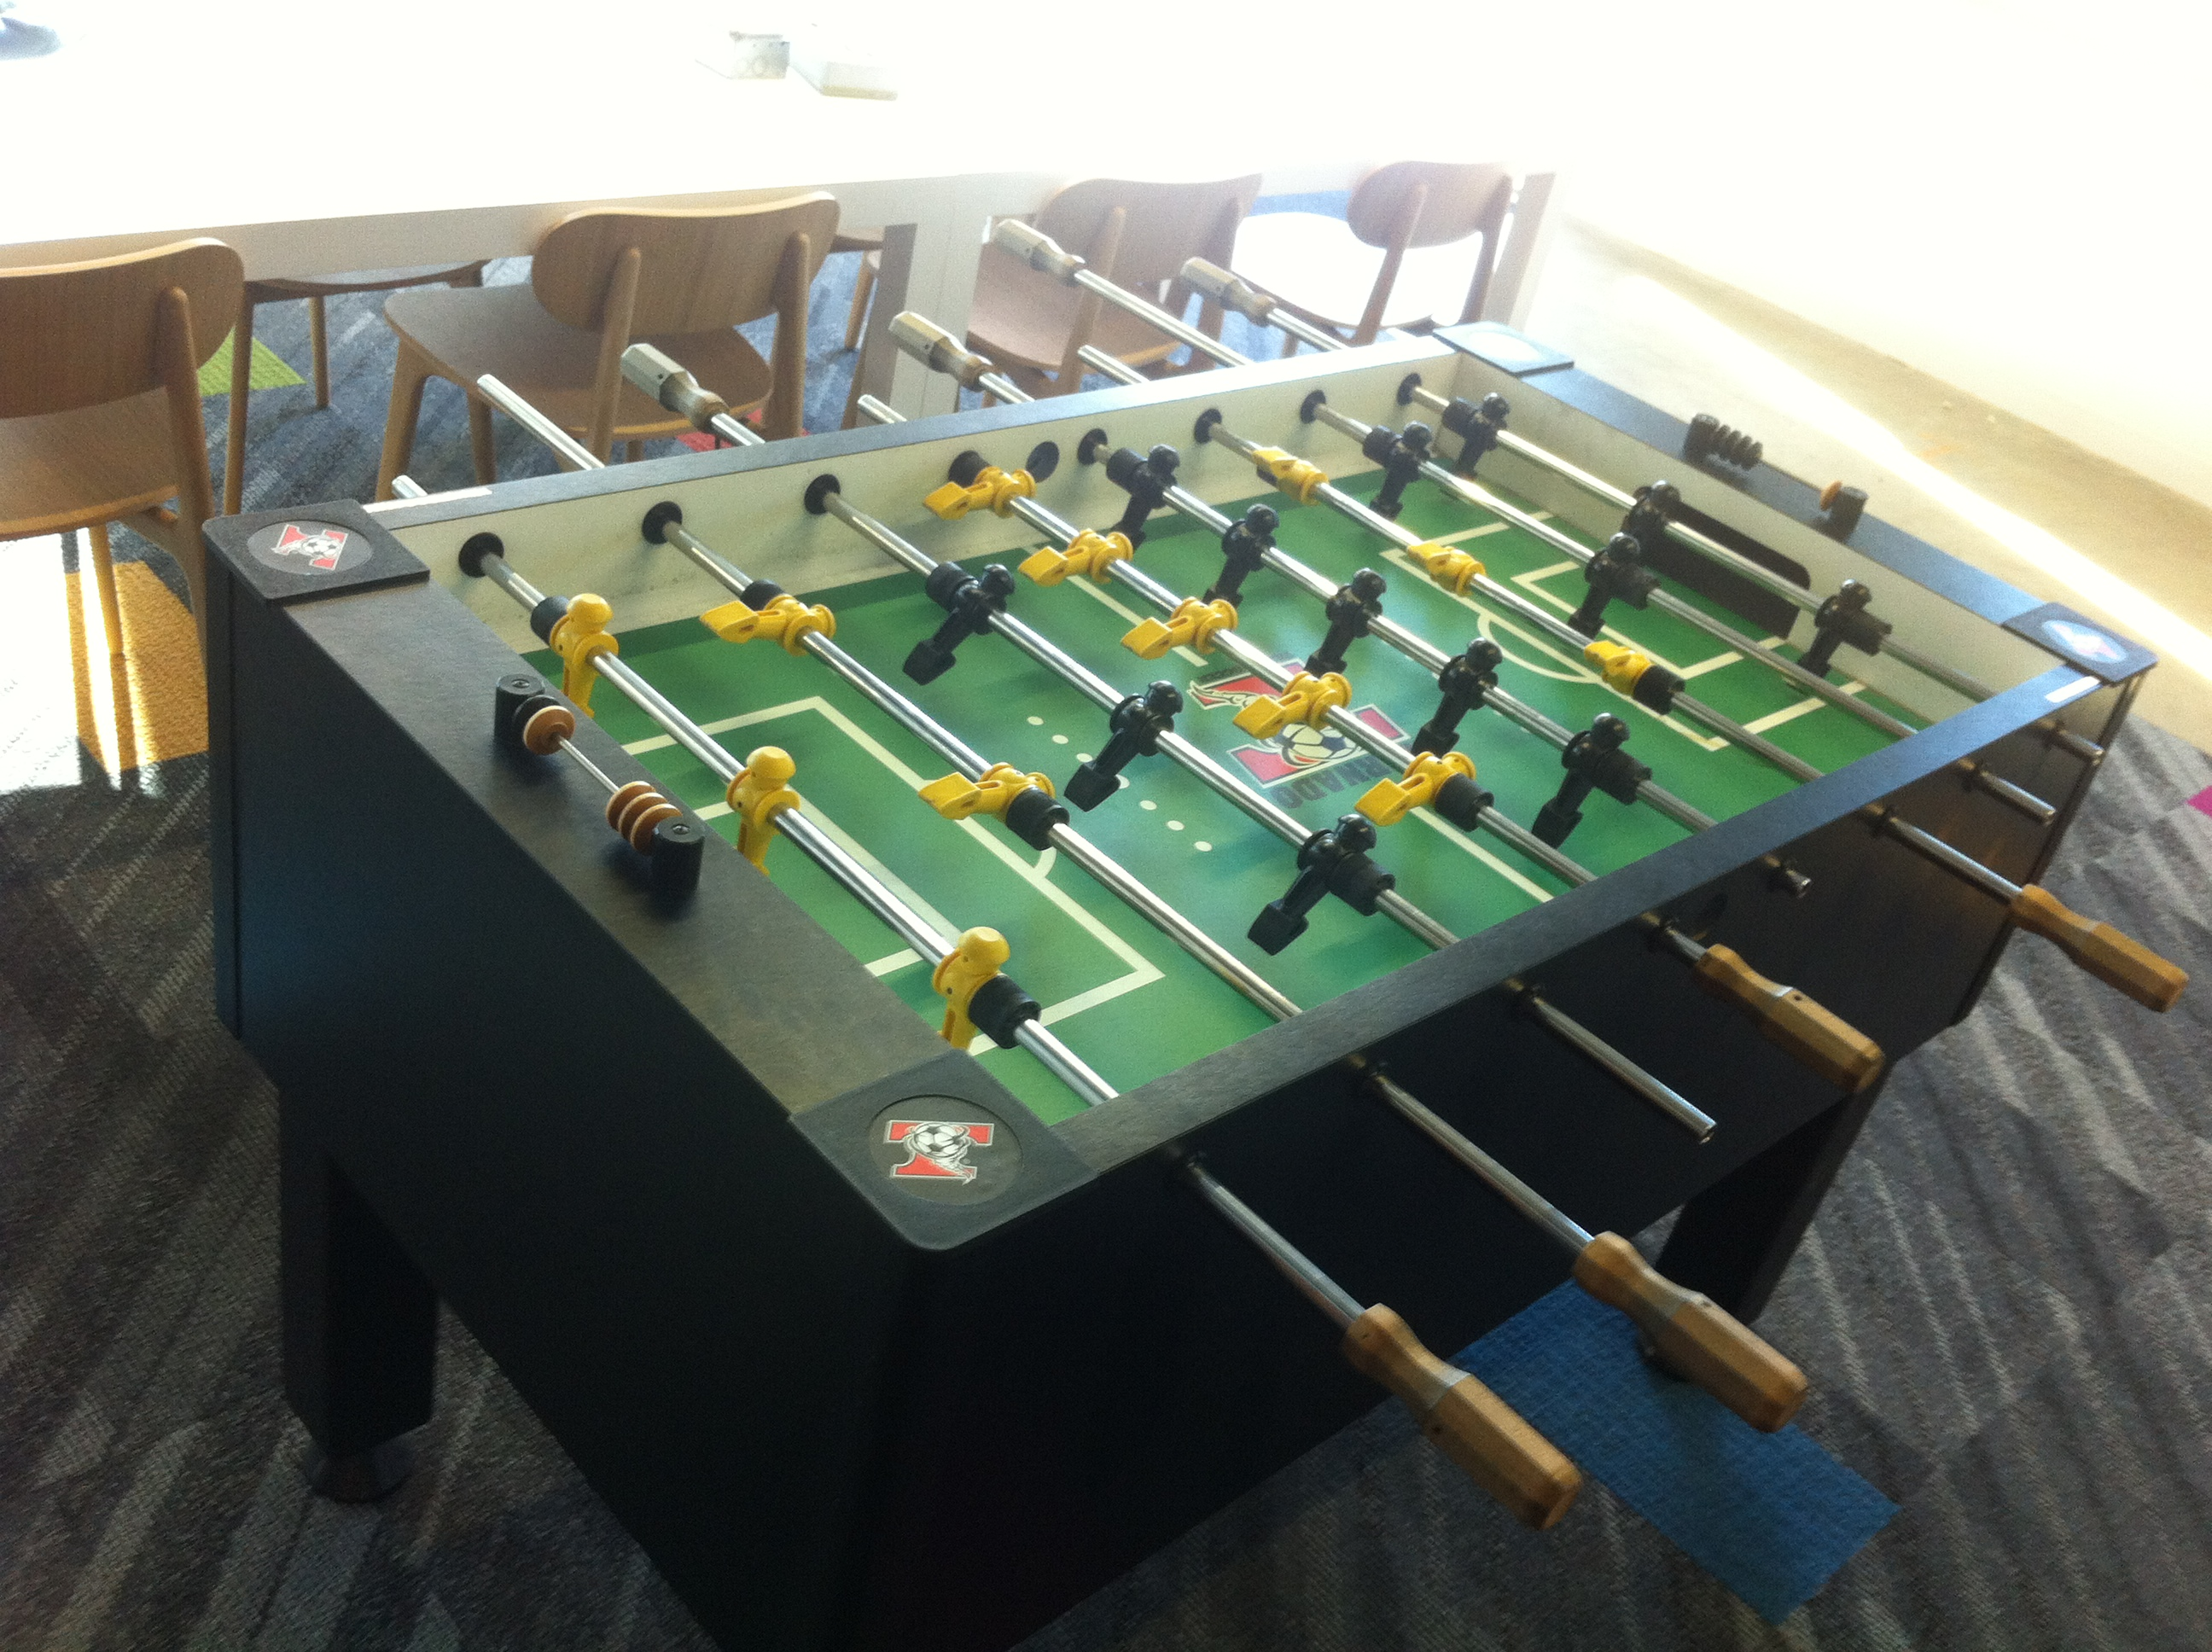
\includegraphics[width=.7\textwidth]{sntc/IMG_2052.JPG}
\end{center}
\end{block}
\end{frame}
\begin{frame}
\frametitle{Competições de Programação}
\begin{block}{Por que é Bom?}
\begin{center}
	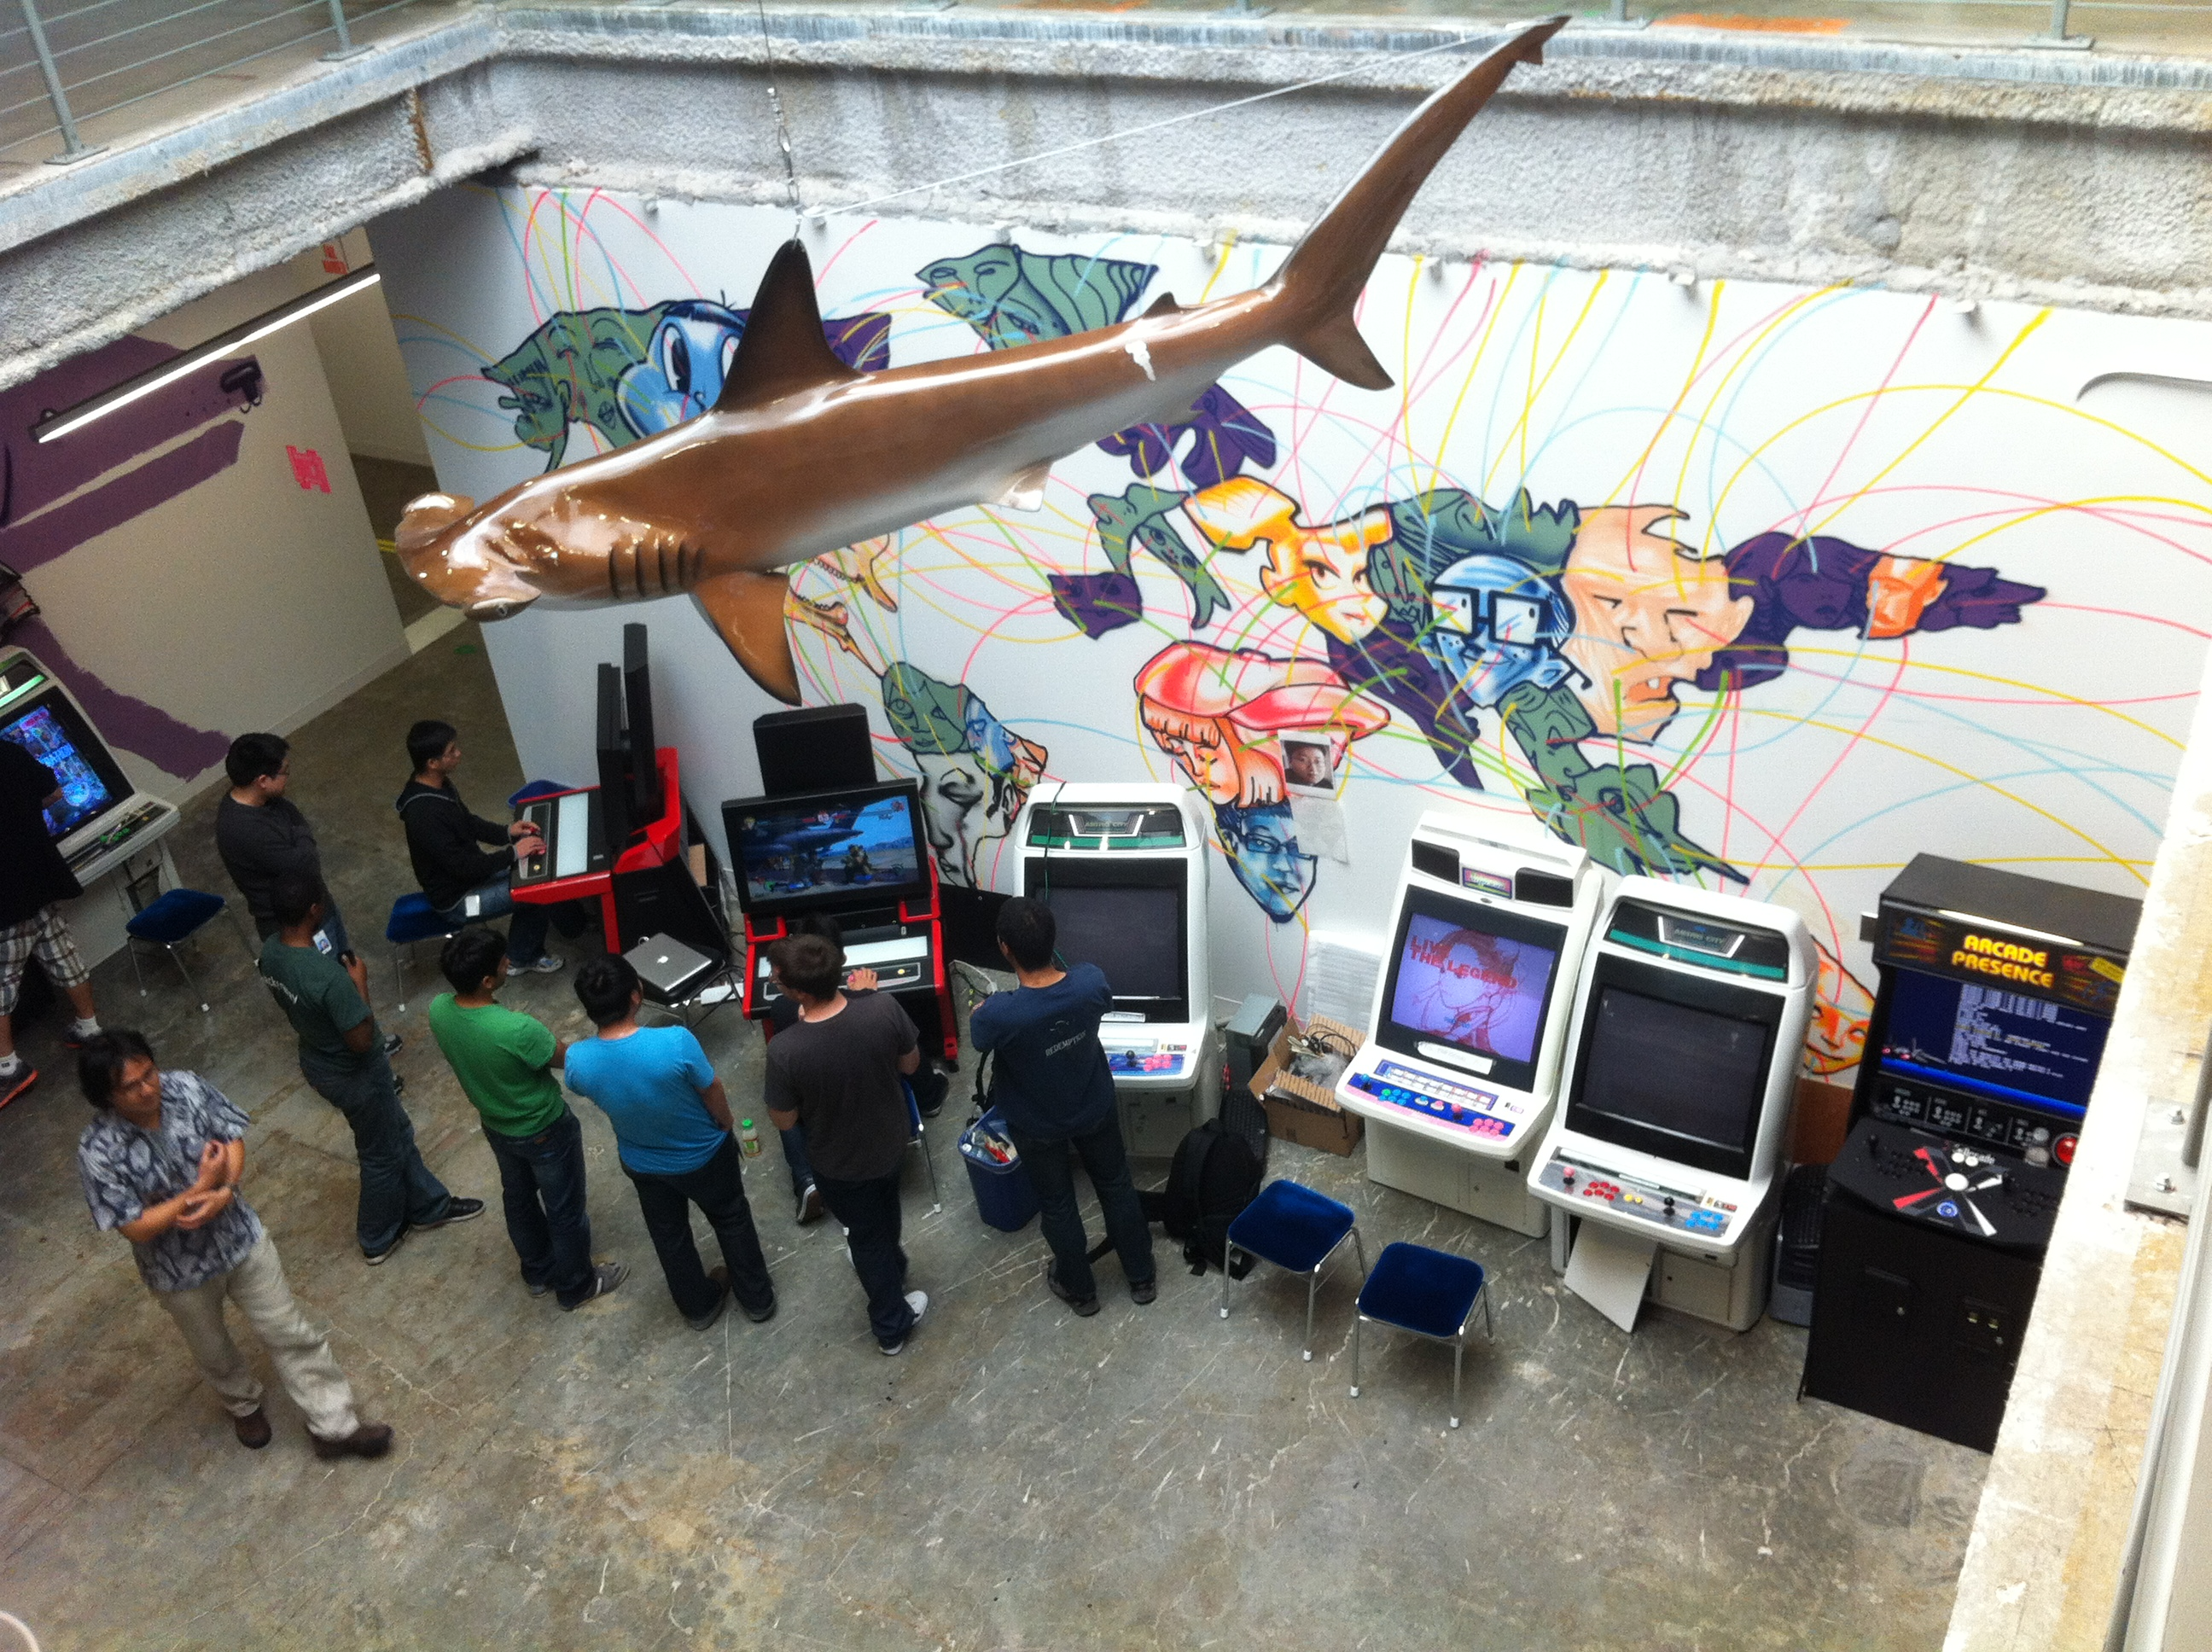
\includegraphics[width=.7\textwidth]{sntc/IMG_2056.JPG}
\end{center}
\end{block}
\end{frame}
\begin{frame}
\frametitle{Competições de Programação}
\begin{block}{Por que é Bom?}
\begin{center}
	
\includegraphics[width=.7\textwidth]{sntc/IMG_2062.JPG}
\end{center}
\end{block}
\end{frame}
\begin{frame}
\frametitle{Competições de Programação}
\begin{block}{Por que é Bom?}
\begin{center}
	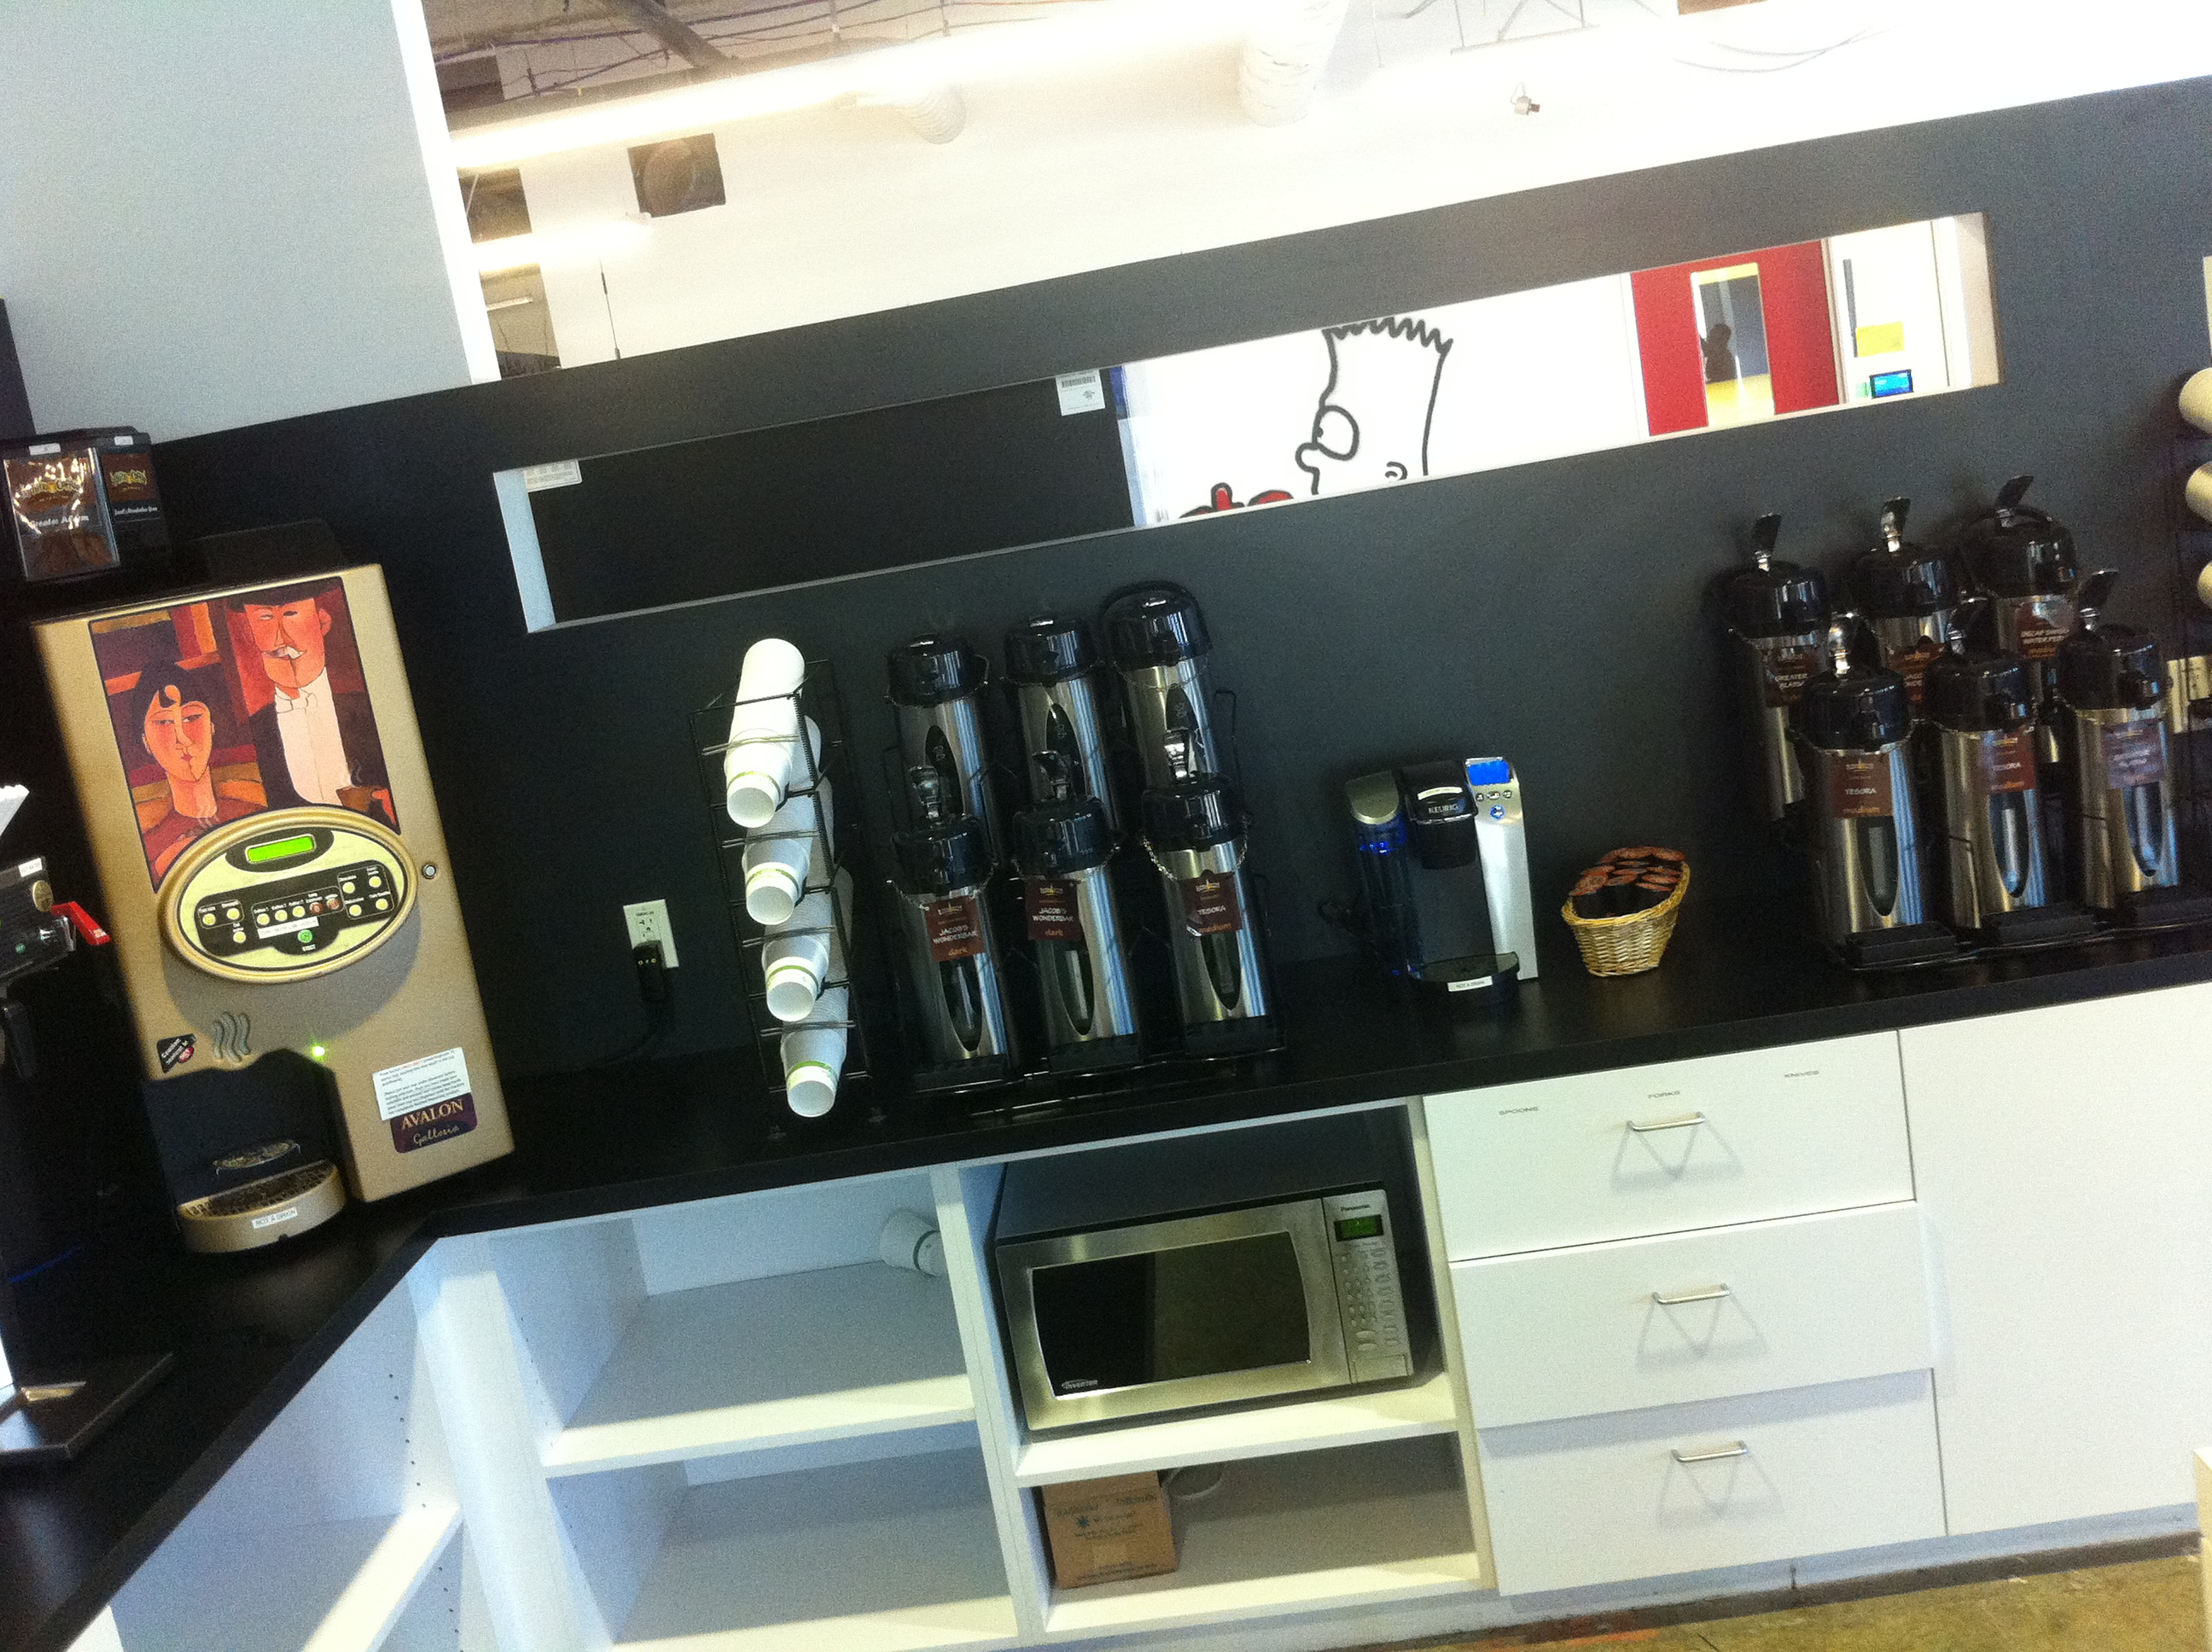
\includegraphics[width=.7\textwidth]{sntc/IMG_2064.JPG}
\end{center}
\end{block}
\end{frame}
\begin{frame}
\frametitle{Competições de Programação}
\begin{block}{Por que é Bom?}
\begin{center}
	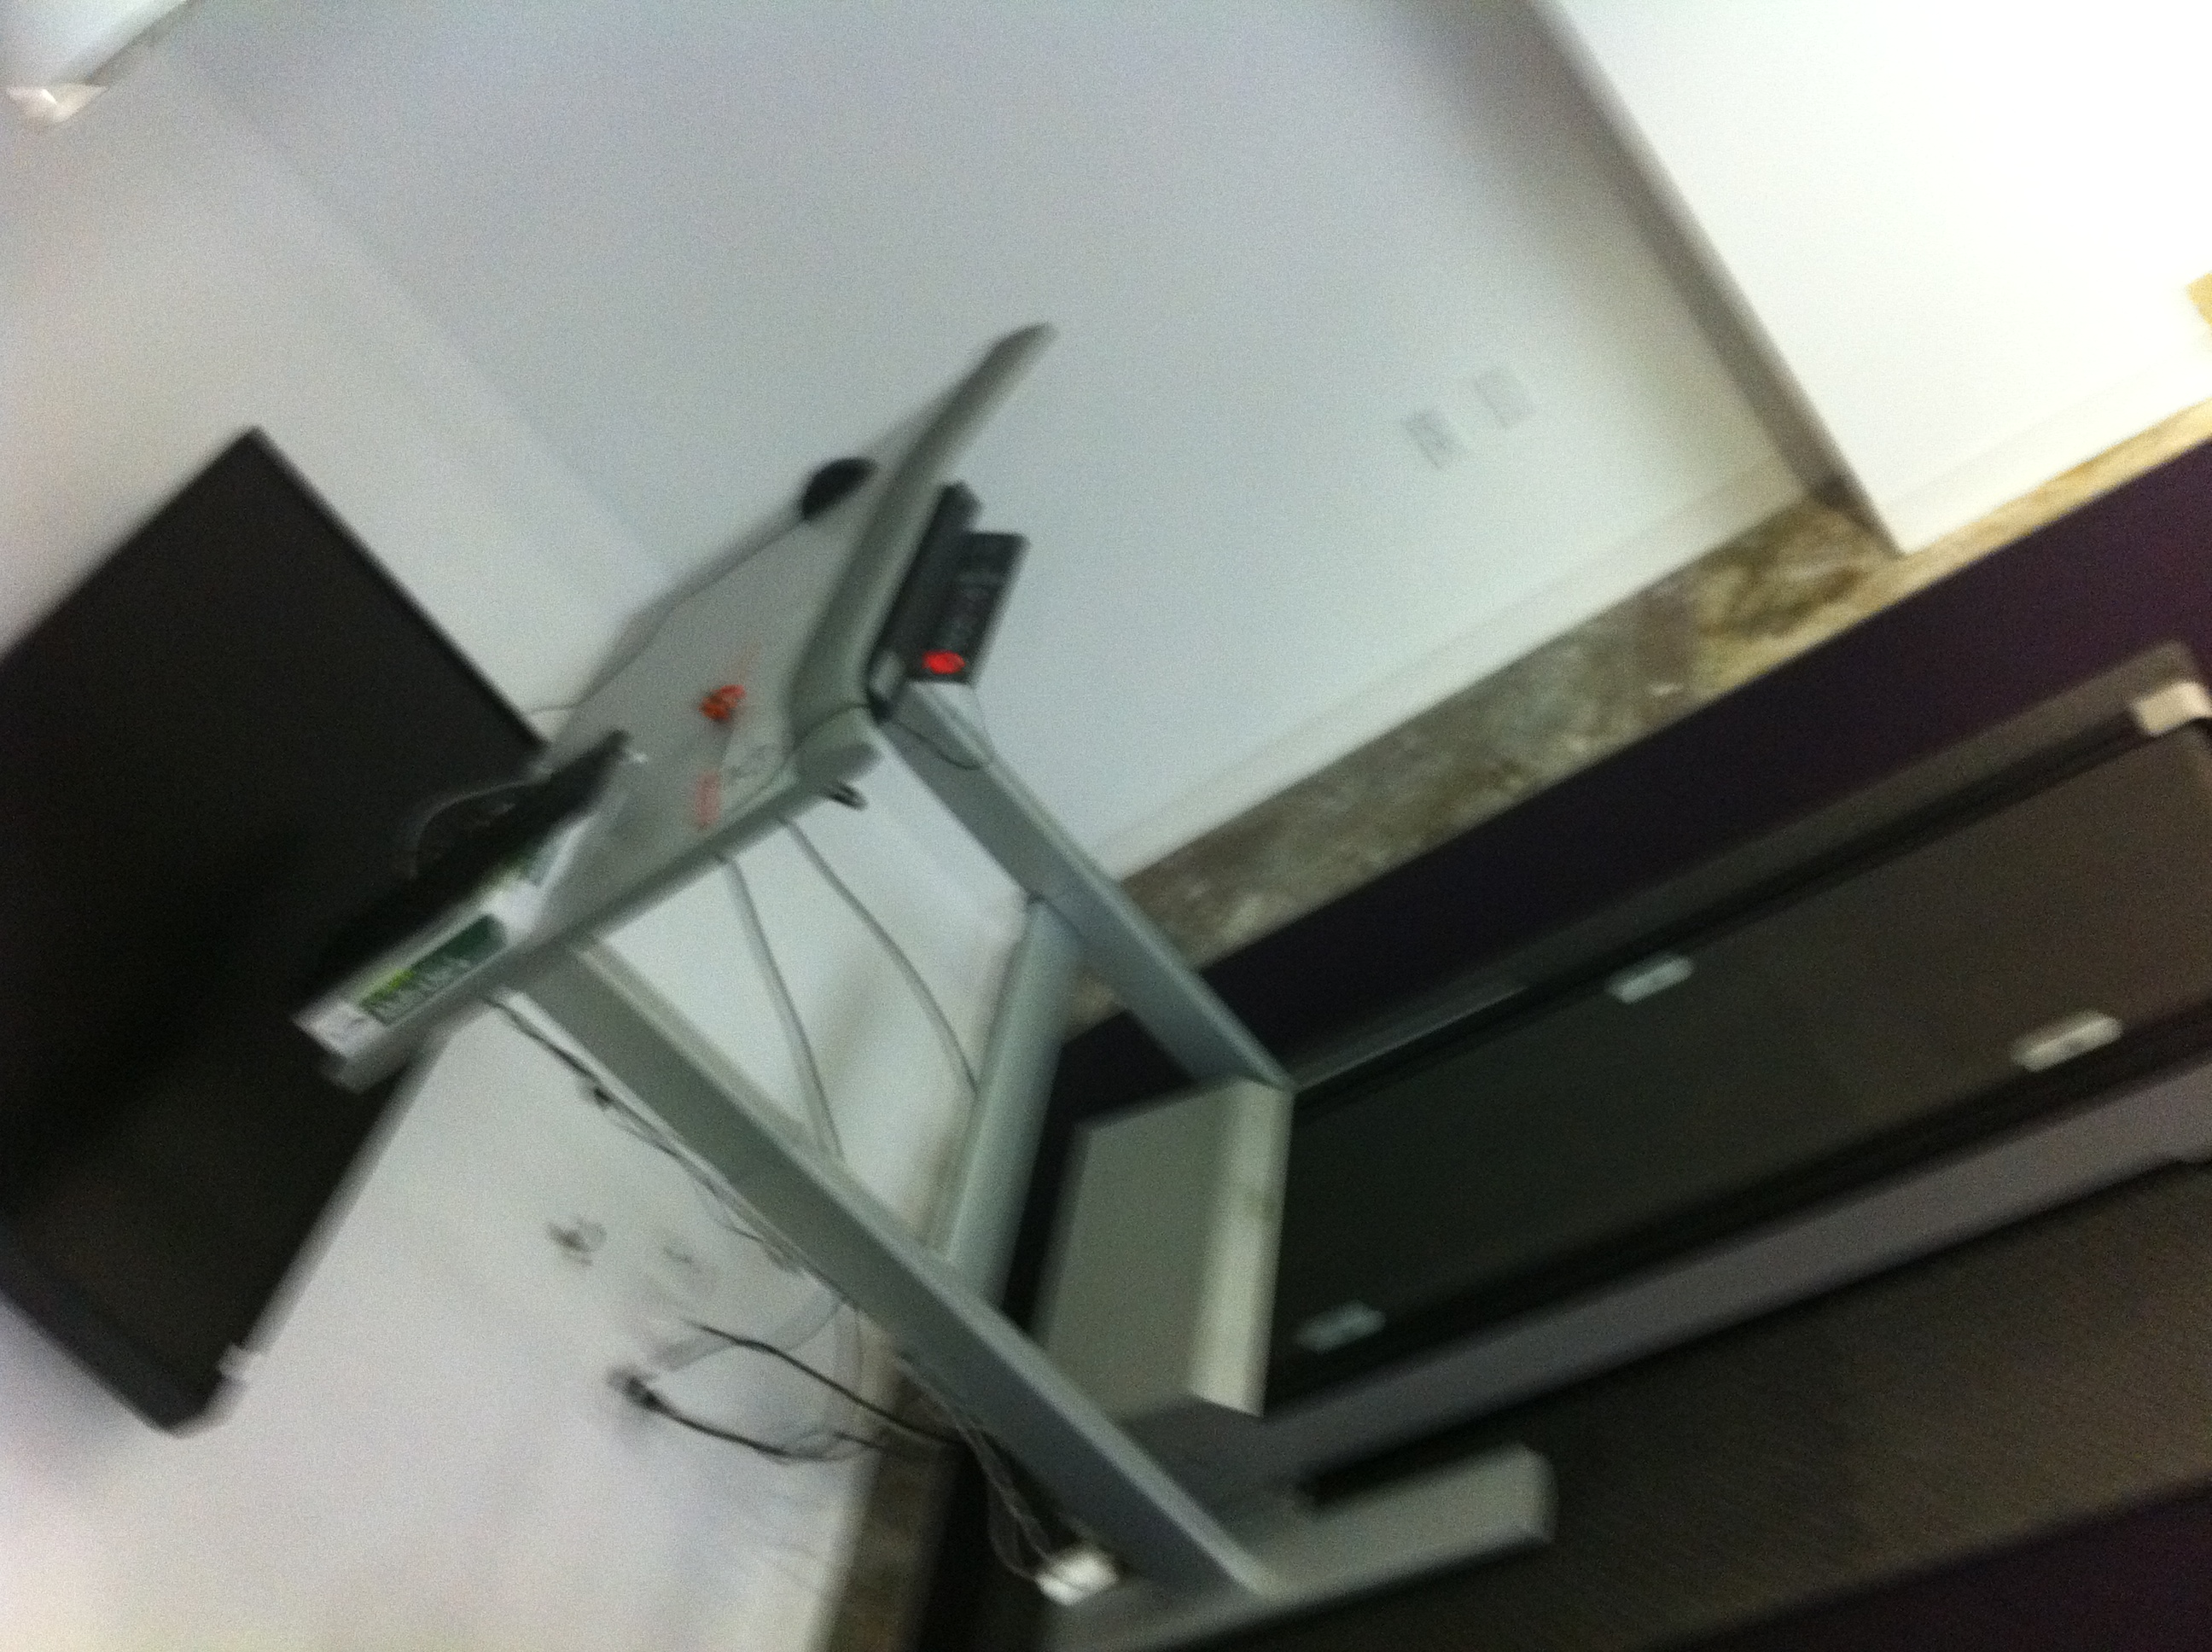
\includegraphics[width=.7\textwidth]{sntc/IMG_2066.JPG}
\end{center}
\end{block}
\end{frame}
\begin{frame}
\frametitle{Competições de Programação}
\begin{block}{Por que é Bom?}
\begin{center}
	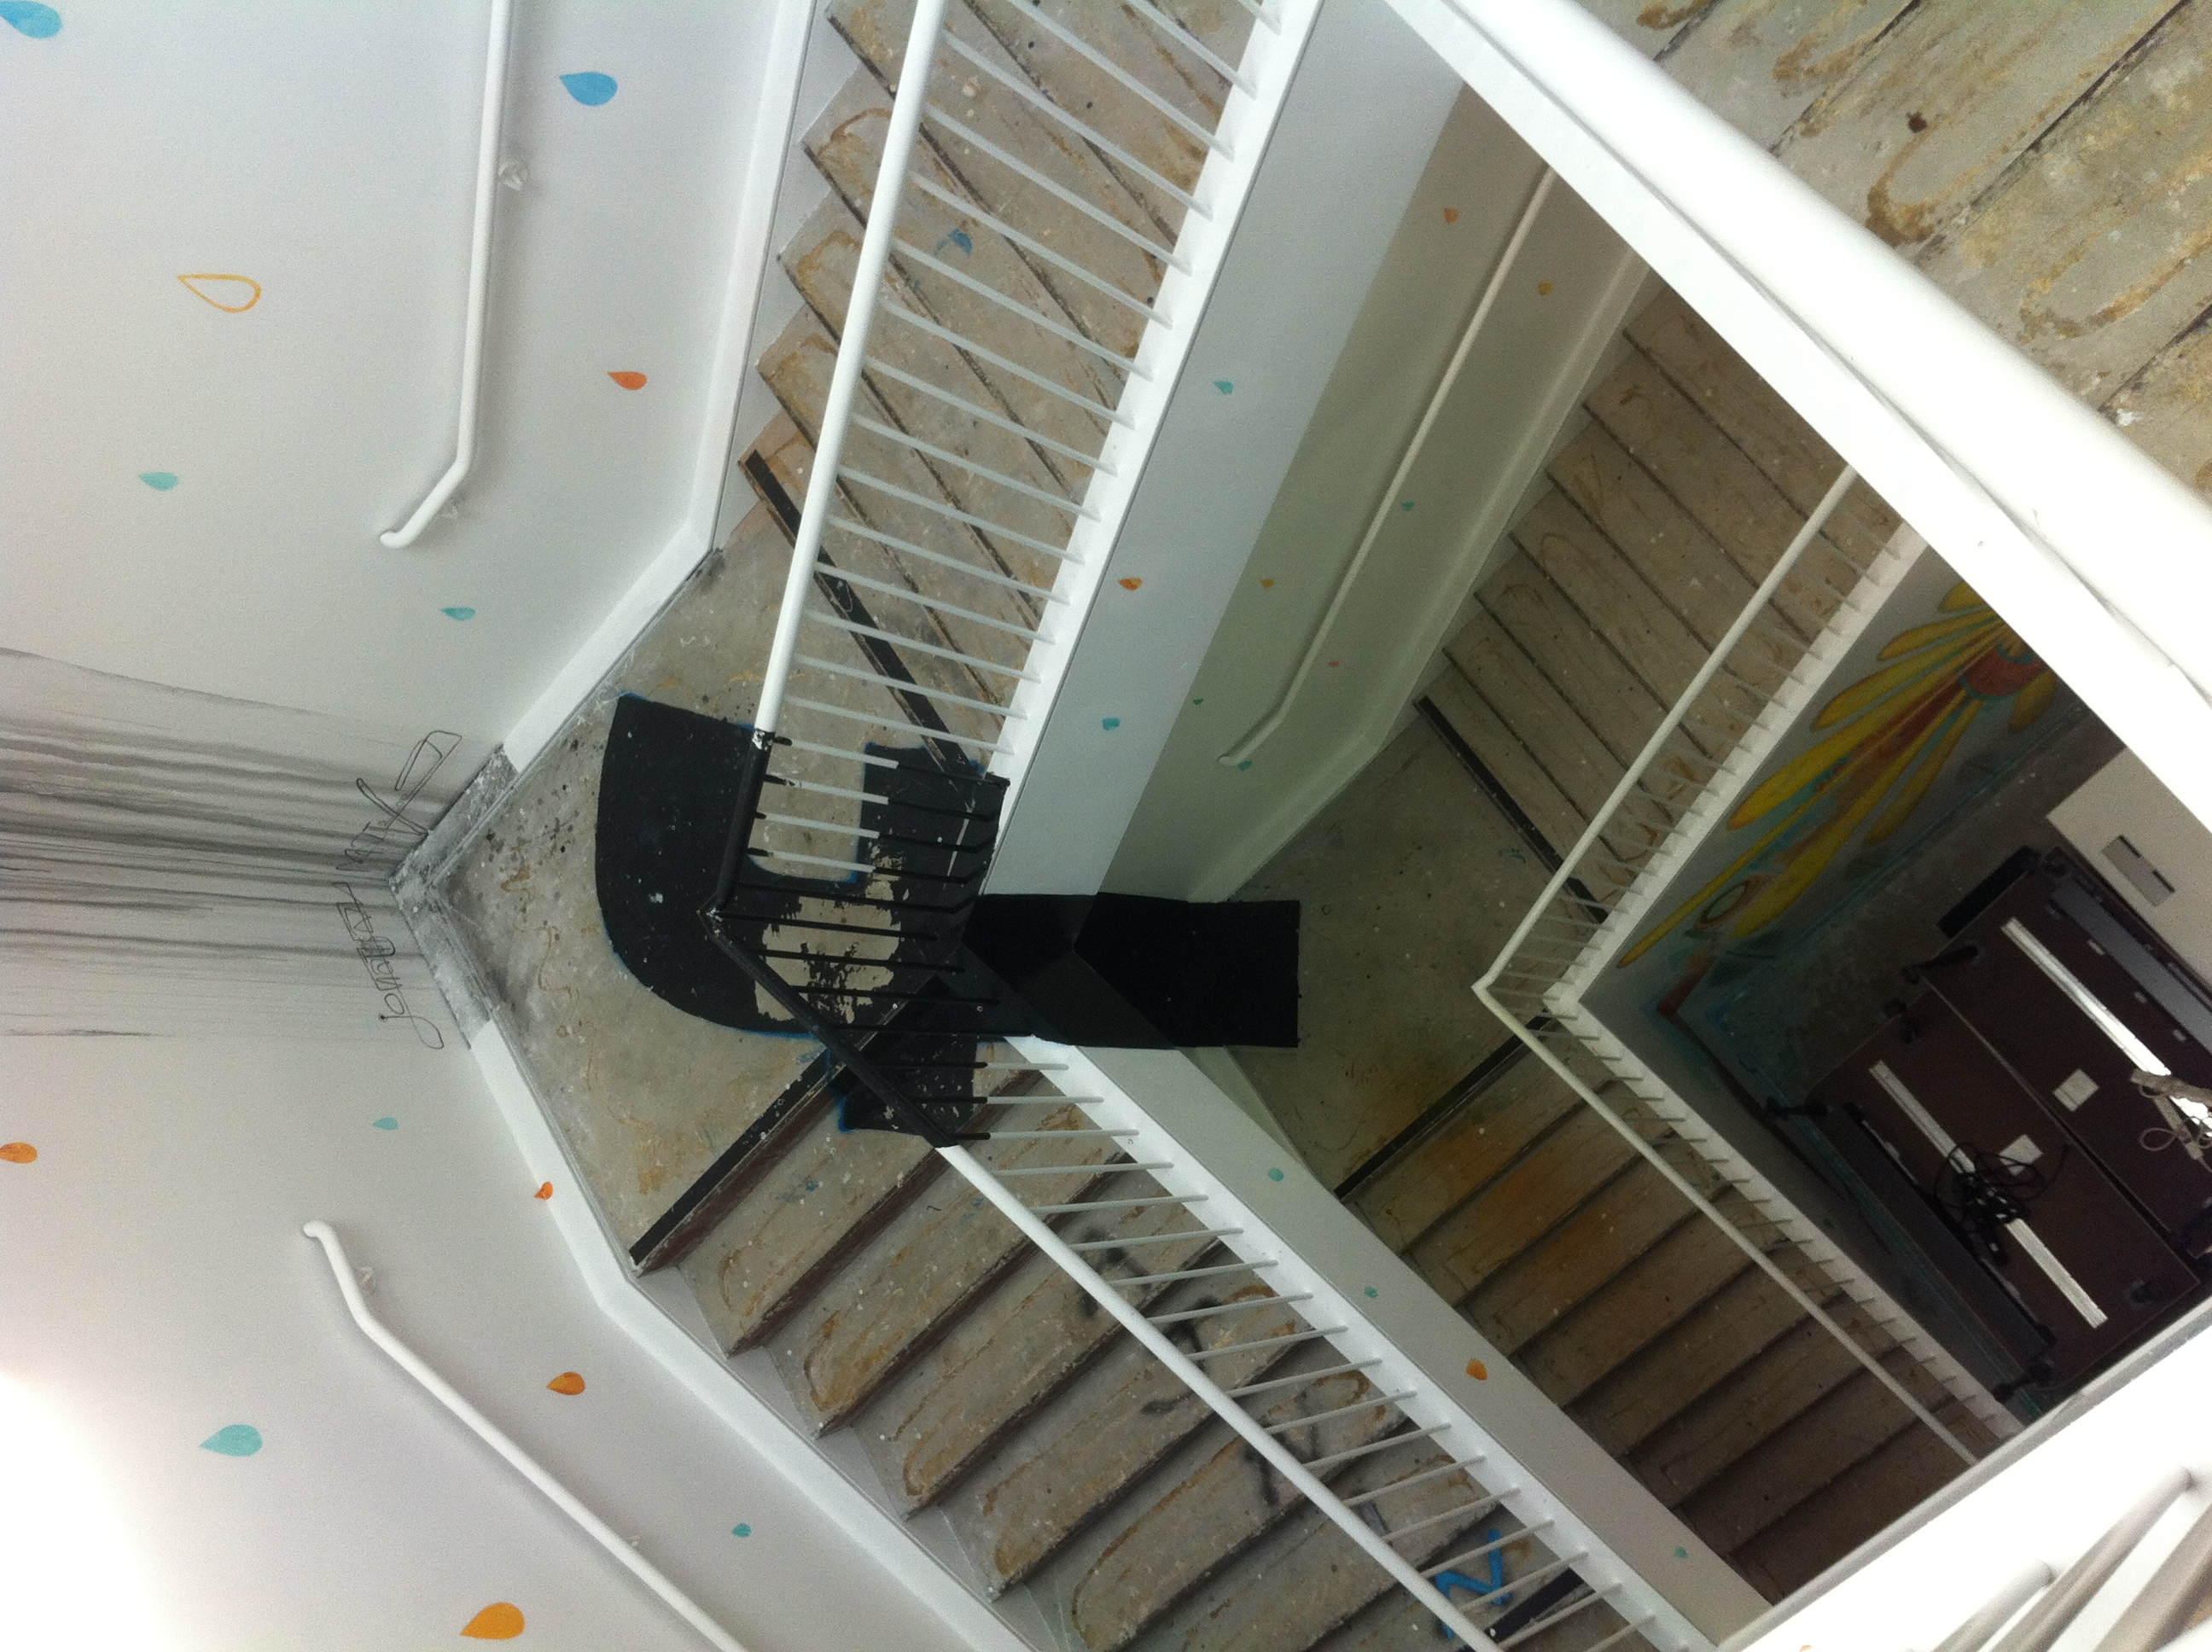
\includegraphics[width=.7\textwidth]{sntc/IMG_2067.JPG}
\end{center}
\end{block}
\end{frame}
\begin{frame}
\frametitle{Competições de Programação}
\begin{block}{Por que é Bom?}
\begin{center}
	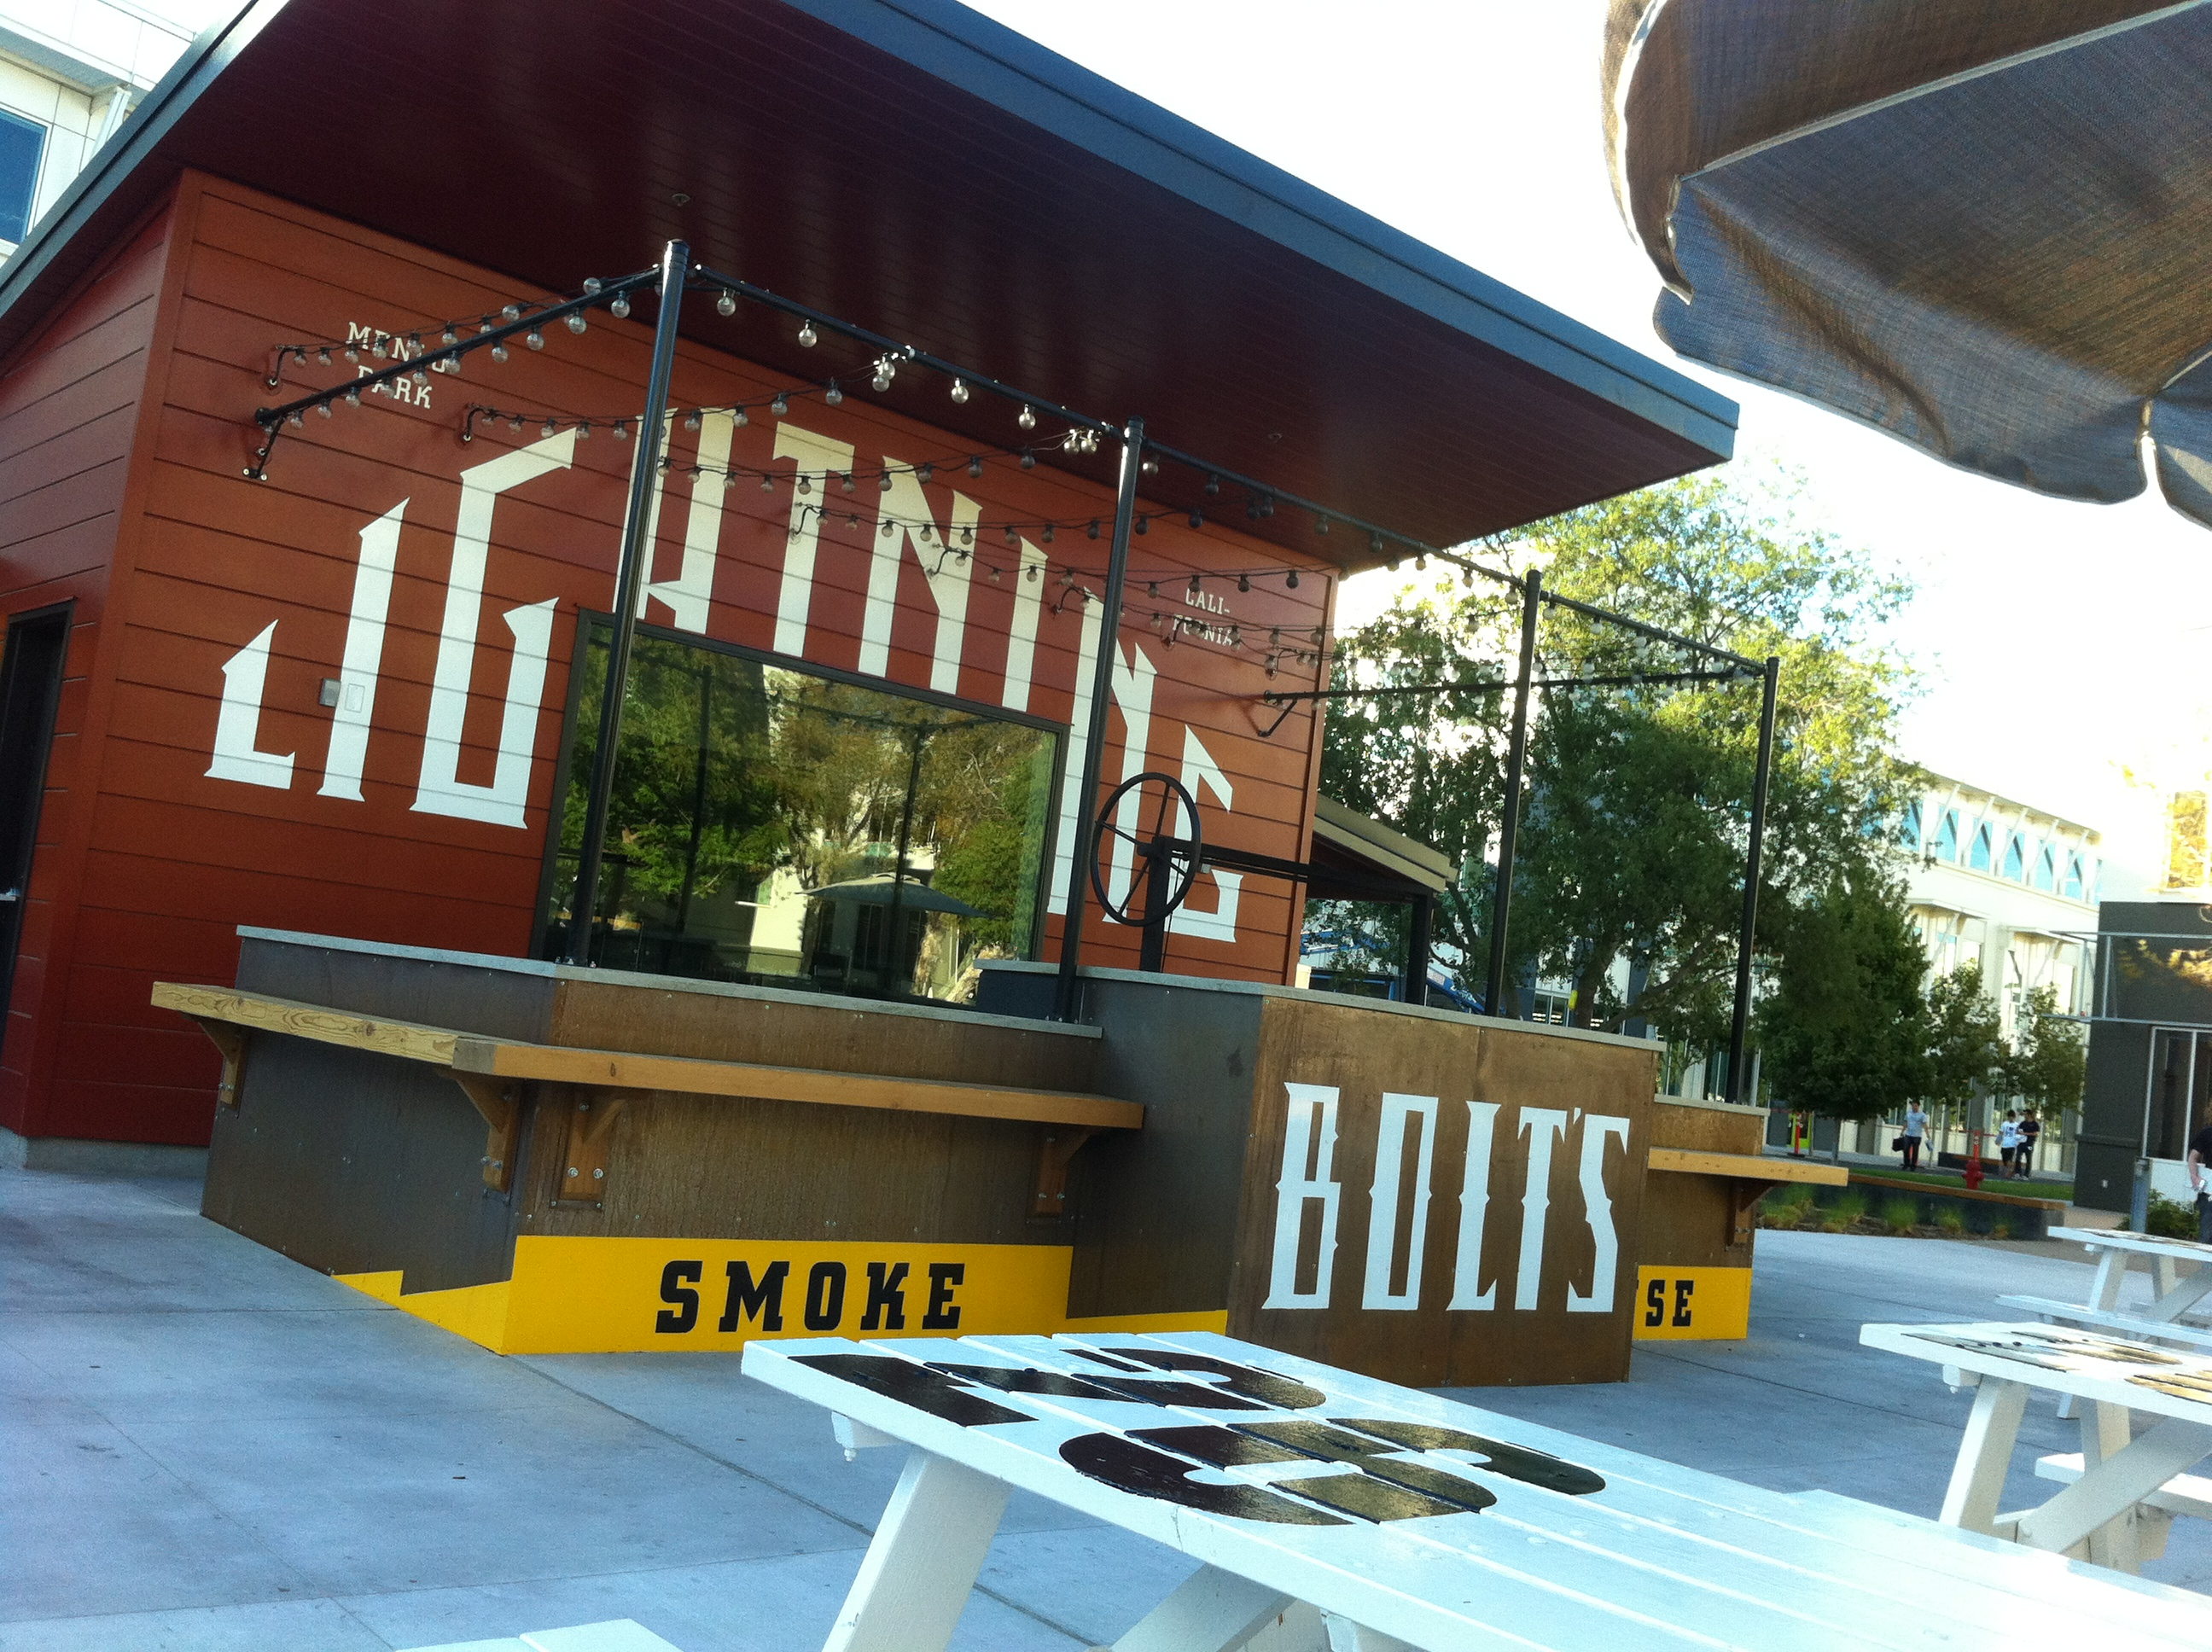
\includegraphics[width=.7\textwidth]{sntc/IMG_2074.JPG}
\end{center}
\end{block}
\end{frame}
\begin{frame}
\frametitle{Competições de Programação}
\begin{block}{Por que é Bom?}
\begin{center}
	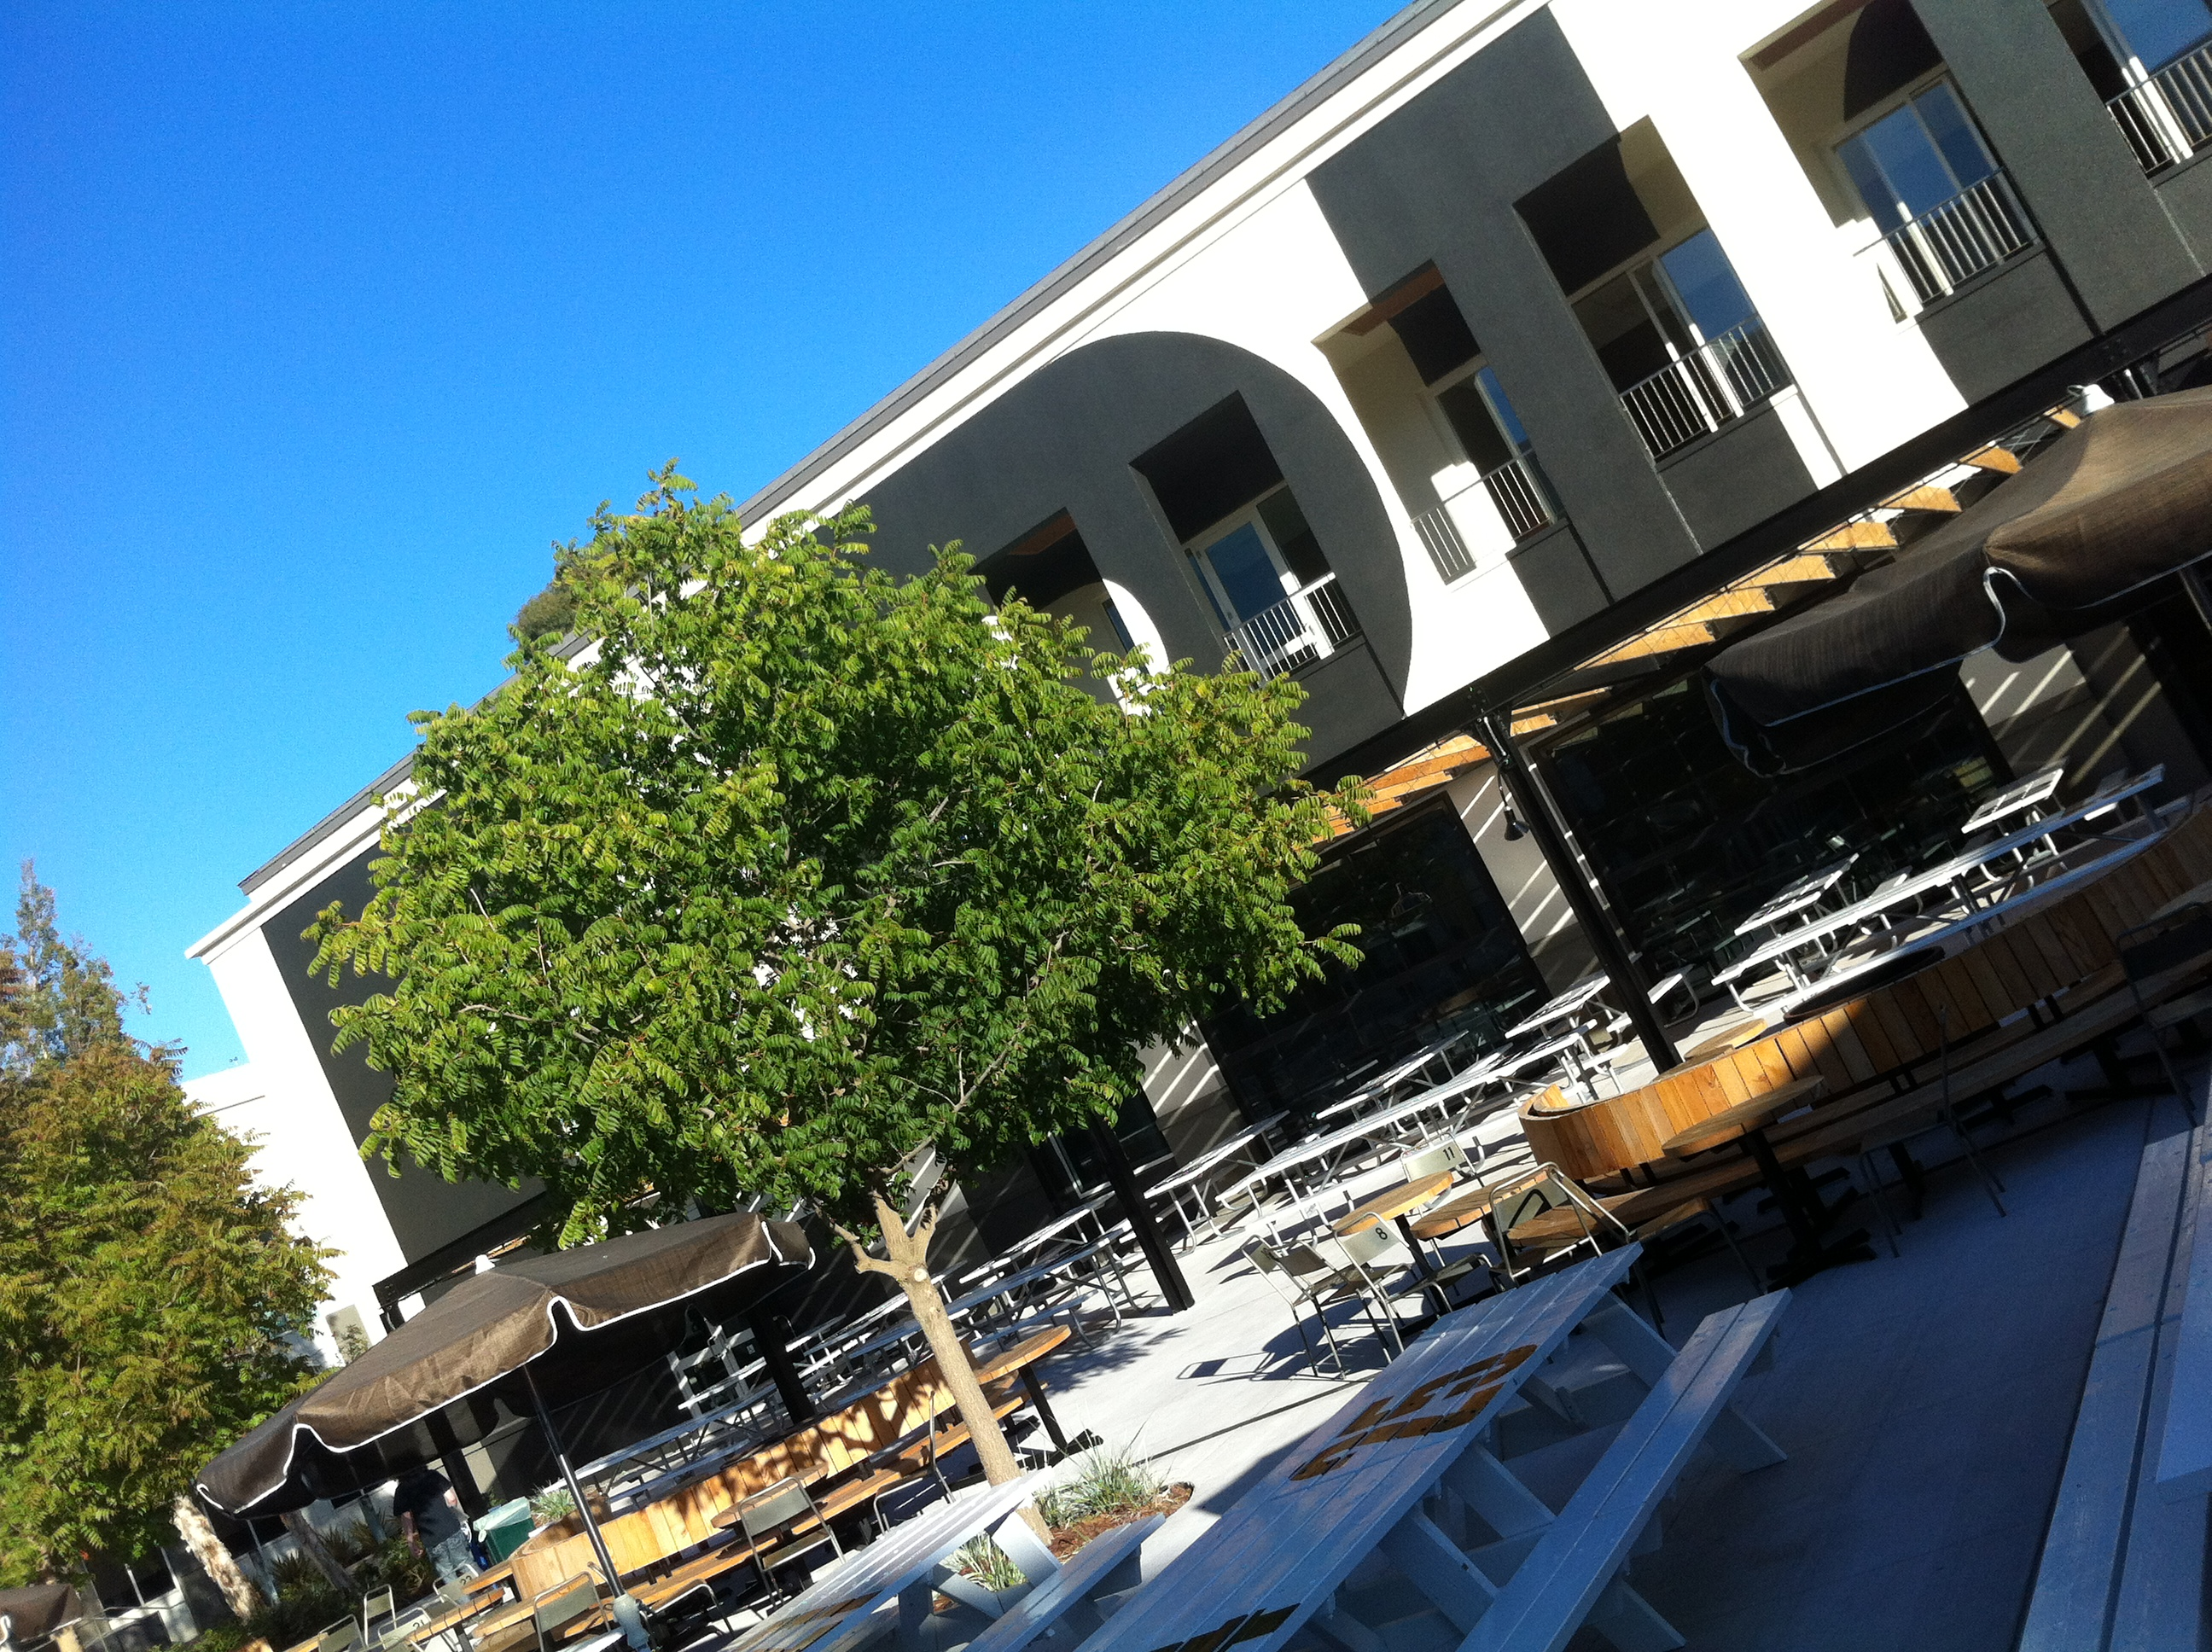
\includegraphics[width=.7\textwidth]{sntc/IMG_2075.JPG}
\end{center}
\end{block}
\end{frame}
%- - - - - - - - - - - - - - - - - - - - - - - - - - - - - - - - - SLIDES - SNCT
%- - - - - - - - - - - - - - - - - - - - - - - - - - - - - - - - -

%- - - - - - - - - - - - - - - - - - - - - - - - - - - - - - - - - SLIDE -
\begin{frame}
\frametitle{Competições de Programação}
\begin{block}{Como funcionam?}
\begin{itemize}
	\item Variam um pouco de estilo e regras, mas em todas é necessário programar.
	\item Existe um tempo fixo para resolver o conjunto de problemas propostos.
	\item Geralmente, para ganhar, você deve resolver o maior número de problemas no menor tempo possível.
\end{itemize}
\end{block}

\end{frame}
%- - - - - - - - - - - - - - - - - - - - - - - - - - - - - - - - - SLIDE -
\begin{frame}
\frametitle{Competições de Programação}
\begin{block}{Algumas competições}
\begin{itemize}
	\item Ensino médio: 
	\begin{itemize}
		\item Olimpíada Brasileira de Informática (OBI)
		\item International Olympiad in Informatics (IOI)
		\item TopCoder High School Tournament (TCHS)
	\end{itemize}
	\item Ensino superior: 
	\begin{itemize}
		\item Maratona de Programação
		\item ACM International Collegiate Programming Contest (ACM-ICPC)
		\item TopCoder Collegiate Challenge (TCCC)
	\end{itemize}
	\item Livre: 
	\begin{itemize}
		\item TopCoder Open (TCO)
		\item Google Code Jam (GCJ)
		\item Facebook Hacker Cup
		\item Internet Problem Solving Contest (IPSC)
		\item $\infty$
	\end{itemize}
\end{itemize}
\end{block}
\end{frame}
%- - - - - - - - - - - - - - - - - - - - - - - - - - - - - - - - - SLIDE -
